\documentclass[journal]{IEEEtran}
%DIF LATEXDIFF DIFFERENCE FILE
%DIF DEL C:\Users\Raymond Tie\AppData\Local\Temp\mart_nilm_baseline_20261028.tex   Sun Nov  8 21:27:17 2026
%DIF ADD multi-applainces_paper.tex                                                Sun Nov  8 21:35:44 2026

\usepackage{cite}
\usepackage{amsmath,amssymb,amsfonts}
\usepackage{algorithm}
\usepackage{algorithmic}
\usepackage{graphicx}
\usepackage{textcomp}
\usepackage{xcolor}
\usepackage{multirow}
\usepackage{tabularx}
\usepackage{booktabs}

%DIF 14a14-32
% Use only ordinary short hyphens throughout the manuscript. %DIF > 
% IEEEtran otherwise inserts em dashes after the Abstract and Index Terms labels %DIF > 
% and an en dash in compressed citation ranges. %DIF > 
\makeatletter %DIF > 
\def\abstract{\normalfont %DIF > 
    \if@twocolumn %DIF > 
      \@IEEEabskeysecsize\bfseries\textit{\abstractname}-\relax %DIF > 
    \else %DIF > 
      \bgroup\par\addvspace{0.5\baselineskip}\centering\vspace{-1.78ex}\@IEEEabskeysecsize\textbf{\abstractname}\par\addvspace{0.5\baselineskip}\egroup\quotation\@IEEEabskeysecsize %DIF > 
    \fi\@IEEEgobbleleadPARNLSP} %DIF > 
\def\IEEEkeywords{\normalfont %DIF > 
    \if@twocolumn %DIF > 
      \@IEEEabskeysecsize\bfseries\textit{\IEEEkeywordsname}-\relax %DIF > 
    \else %DIF > 
      \bgroup\par\addvspace{0.5\baselineskip}\centering\@IEEEabskeysecsize\textbf{\IEEEkeywordsname}\par\addvspace{0.5\baselineskip}\egroup\quotation\@IEEEabskeysecsize %DIF > 
    \fi\@IEEEgobbleleadPARNLSP} %DIF > 
\def\citedash{]-[} %DIF > 
\makeatother %DIF > 
 %DIF > 
%DIF -------

% Mean and standard deviation stacked in two rows with matching font size.
\newcommand{\mstd}[2]{\shortstack{#1\\[-2pt]{$\pm$#2}}}
\newcommand{\bestmstd}[2]{{\bfseries\shortstack{#1\\[-2pt]{$\boldsymbol{\pm}$#2}}}}
%DIF PREAMBLE EXTENSION ADDED BY LATEXDIFF
%DIF CFONT PREAMBLE %DIF PREAMBLE
\RequirePackage{color}\definecolor{RED}{rgb}{1,0,0}\definecolor{BLUE}{rgb}{0,0,1} %DIF PREAMBLE
\DeclareOldFontCommand{\sf}{\normalfont\sffamily}{\mathsf} %DIF PREAMBLE
\providecommand{\DIFadd}[1]{{\protect\color{blue} \sf #1}} %DIF PREAMBLE
\providecommand{\DIFdel}[1]{{\protect\color{red} \scriptsize #1}} %DIF PREAMBLE
%DIF SAFE PREAMBLE %DIF PREAMBLE
\providecommand{\DIFaddbegin}{} %DIF PREAMBLE
\providecommand{\DIFaddend}{} %DIF PREAMBLE
\providecommand{\DIFdelbegin}{} %DIF PREAMBLE
\providecommand{\DIFdelend}{} %DIF PREAMBLE
\providecommand{\DIFmodbegin}{} %DIF PREAMBLE
\providecommand{\DIFmodend}{} %DIF PREAMBLE
%DIF FLOATSAFE PREAMBLE %DIF PREAMBLE
\providecommand{\DIFaddFL}[1]{\DIFadd{#1}} %DIF PREAMBLE
\providecommand{\DIFdelFL}[1]{\DIFdel{#1}} %DIF PREAMBLE
\providecommand{\DIFaddbeginFL}{} %DIF PREAMBLE
\providecommand{\DIFaddendFL}{} %DIF PREAMBLE
\providecommand{\DIFdelbeginFL}{} %DIF PREAMBLE
\providecommand{\DIFdelendFL}{} %DIF PREAMBLE
\providecommand{\DIFscaledelfig}{0.5}
%DIF HIGHLIGHTGRAPHICS PREAMBLE %DIF PREAMBLE
\RequirePackage{settobox} %DIF PREAMBLE
\RequirePackage{letltxmacro} %DIF PREAMBLE
\newsavebox{\DIFdelgraphicsbox} %DIF PREAMBLE
\newlength{\DIFdelgraphicswidth} %DIF PREAMBLE
\newlength{\DIFdelgraphicsheight} %DIF PREAMBLE
% store original definition of \includegraphics %DIF PREAMBLE
\LetLtxMacro{\DIFOincludegraphics}{\includegraphics} %DIF PREAMBLE
\providecommand{\DIFaddincludegraphics}[2][]{{\color{blue}\fbox{\DIFOincludegraphics[#1]{#2}}}} %DIF PREAMBLE
\providecommand{\DIFdelincludegraphics}[2][]{% %DIF PREAMBLE
\sbox{\DIFdelgraphicsbox}{\DIFOincludegraphics[#1]{#2}}% %DIF PREAMBLE
\settoboxwidth{\DIFdelgraphicswidth}{\DIFdelgraphicsbox} %DIF PREAMBLE
\settoboxtotalheight{\DIFdelgraphicsheight}{\DIFdelgraphicsbox} %DIF PREAMBLE
\scalebox{\DIFscaledelfig}{% %DIF PREAMBLE
\parbox[b]{\DIFdelgraphicswidth}{\usebox{\DIFdelgraphicsbox}\\[-\baselineskip] \rule{\DIFdelgraphicswidth}{0em}}\llap{\resizebox{\DIFdelgraphicswidth}{\DIFdelgraphicsheight}{% %DIF PREAMBLE
\setlength{\unitlength}{\DIFdelgraphicswidth}% %DIF PREAMBLE
\begin{picture}(1,1)% %DIF PREAMBLE
\thicklines\linethickness{2pt} %DIF PREAMBLE
{\color[rgb]{1,0,0}\put(0,0){\framebox(1,1){}}}% %DIF PREAMBLE
{\color[rgb]{1,0,0}\put(0,0){\line( 1,1){1}}}% %DIF PREAMBLE
{\color[rgb]{1,0,0}\put(0,1){\line(1,-1){1}}}% %DIF PREAMBLE
\end{picture}% %DIF PREAMBLE
}\hspace*{3pt}}} %DIF PREAMBLE
} %DIF PREAMBLE
\LetLtxMacro{\DIFOaddbegin}{\DIFaddbegin} %DIF PREAMBLE
\LetLtxMacro{\DIFOaddend}{\DIFaddend} %DIF PREAMBLE
\LetLtxMacro{\DIFOdelbegin}{\DIFdelbegin} %DIF PREAMBLE
\LetLtxMacro{\DIFOdelend}{\DIFdelend} %DIF PREAMBLE
\DeclareRobustCommand{\DIFaddbegin}{\DIFOaddbegin \let\includegraphics\DIFaddincludegraphics} %DIF PREAMBLE
\DeclareRobustCommand{\DIFaddend}{\DIFOaddend \let\includegraphics\DIFOincludegraphics} %DIF PREAMBLE
\DeclareRobustCommand{\DIFdelbegin}{\DIFOdelbegin \let\includegraphics\DIFdelincludegraphics} %DIF PREAMBLE
\DeclareRobustCommand{\DIFdelend}{\DIFOaddend \let\includegraphics\DIFOincludegraphics} %DIF PREAMBLE
\LetLtxMacro{\DIFOaddbeginFL}{\DIFaddbeginFL} %DIF PREAMBLE
\LetLtxMacro{\DIFOaddendFL}{\DIFaddendFL} %DIF PREAMBLE
\LetLtxMacro{\DIFOdelbeginFL}{\DIFdelbeginFL} %DIF PREAMBLE
\LetLtxMacro{\DIFOdelendFL}{\DIFdelendFL} %DIF PREAMBLE
\DeclareRobustCommand{\DIFaddbeginFL}{\DIFOaddbeginFL \let\includegraphics\DIFaddincludegraphics} %DIF PREAMBLE
\DeclareRobustCommand{\DIFaddendFL}{\DIFOaddendFL \let\includegraphics\DIFOincludegraphics} %DIF PREAMBLE
\DeclareRobustCommand{\DIFdelbeginFL}{\DIFOdelbeginFL \let\includegraphics\DIFdelincludegraphics} %DIF PREAMBLE
\DeclareRobustCommand{\DIFdelendFL}{\DIFOaddendFL \let\includegraphics\DIFOincludegraphics} %DIF PREAMBLE
%DIF COLORLISTINGS PREAMBLE %DIF PREAMBLE
\RequirePackage{listings} %DIF PREAMBLE
\RequirePackage{color} %DIF PREAMBLE
\lstdefinelanguage{DIFcode}{ %DIF PREAMBLE
%DIF DIFCODE_CFONT %DIF PREAMBLE
  moredelim=[il][\color{red}\scriptsize]{\%DIF\ <\ }, %DIF PREAMBLE
  moredelim=[il][\color{blue}\sffamily]{\%DIF\ >\ } %DIF PREAMBLE
} %DIF PREAMBLE
\lstdefinestyle{DIFverbatimstyle}{ %DIF PREAMBLE
	language=DIFcode, %DIF PREAMBLE
	basicstyle=\ttfamily, %DIF PREAMBLE
	columns=fullflexible, %DIF PREAMBLE
	keepspaces=true %DIF PREAMBLE
} %DIF PREAMBLE
\lstnewenvironment{DIFverbatim}[1][]{\lstset{style=DIFverbatimstyle}}{} %DIF PREAMBLE
\lstnewenvironment{DIFverbatim*}[1][]{\lstset{style=DIFverbatimstyle,showspaces=true}}{} %DIF PREAMBLE
\lstset{extendedchars=\true,inputencoding=utf8}

%DIF END PREAMBLE EXTENSION ADDED BY LATEXDIFF

\begin{document}

\title{MART-NILM: A Compact Multi-Appliance Representation Temporal Network for Joint Power-\DIFdelbegin \DIFdel{-}\DIFdelend State Estimation in Non-Intrusive Load Monitoring}

\author{Raymond \DIFdelbegin \DIFdel{Tie }\DIFdelend Siou Hin \DIFaddbegin \DIFadd{Tie}\DIFaddend , \DIFaddbegin \DIFadd{Wen-Shan }\DIFaddend Tan\DIFdelbegin \DIFdel{Wen Shan}\DIFdelend , \DIFdelbegin \DIFdel{Ding }\DIFdelend Ze Yang \DIFaddbegin \DIFadd{Ding}\DIFaddend ,
Mirza Rayana Sanzana, and Haval Kamil%
\DIFdelbegin %DIFDELCMD < \thanks{Raymond Tie Siou Hin, Tan Wen Shan, and Ding Ze Yang are with the
%DIFDELCMD < Department of Electrical and Robotics and the Centre for Net-Zero Technology,
%DIFDELCMD < Monash University Malaysia, Bandar Sunway, Malaysia
%DIFDELCMD < (e-mail: tan.wenshan@monash.edu).}%%%
\DIFdelend \DIFaddbegin \thanks{Raymond Siou Hin Tie, Wen-Shan Tan, and Ze Yang Ding are with the
Department of Electrical and Robotics and the Centre for Net-Zero Technology,
Monash University Malaysia, Bandar Sunway, Malaysia
(e-mail: tan.wenshan@monash.edu).}\DIFaddend %
\thanks{Mirza Rayana Sanzana is with the School of Information Technology,
Monash University Malaysia, Bandar Sunway, Malaysia.}%
\thanks{Haval Kamil is with the Department of Air Conditioning and
Refrigeration, College of Engineering Technology, Al-Kitab University,
Kirkuk, Iraq.}}

\maketitle

\begin{abstract}
Joint multi-appliance non-intrusive load monitoring (NILM) estimates appliance power and multi-label ON-OFF states from aggregate measurements using a single model. However, compact joint learning is challenged by sparse appliance activations observed under limited background-demand conditions and unequal power-state loss scales across appliances. This paper proposes the Multi-Appliance Representation Temporal Network for NILM (MART-NILM), combining shared temporal encoding, appliance-specific decoding, and cross-appliance feature exchange. Two training-only strategies address these challenges. Focal-event background-stratified mixing pairs selected ON-event traces with recorded residual backgrounds sampled across power strata, while bounded appliance-wise balancing calibrates power and state loss contributions separately for each appliance. Experiments on the UK Domestic Appliance-Level Electricity (UK-DALE) and REFIT datasets, with disjoint training, validation, and test houses, show that MART-NILM outperforms three reproduced joint multi-appliance baselines in appliance-average power error and macro-F1. It achieves mean absolute errors of 7.3 and 10.9~W and macro-F1 scores of 0.88 and 0.72, respectively. Compared with the strongest baseline, ON-state mean absolute error decreases by 58.4\% and 34.4\%, with 54.6\% fewer parameters (1.373 million). These results support an improved accuracy-capacity trade-off for joint residential appliance monitoring.
\end{abstract}

\begin{IEEEkeywords}
Energy disaggregation, multi-appliance estimation, multi-label classification, multi-task learning, non-intrusive load monitoring, power-state estimation.
\end{IEEEkeywords}

\section{Introduction}

Effective residential demand-side management requires appliance-level visibility into both electricity consumption and operating states. Power estimates quantify appliance demand, whereas state estimates expose activation timing; aggregate metering reveals neither directly. Appliance-level feedback can support energy conservation~\cite{delmas2013information}, but dedicated submetering requires installing and maintaining additional sensors. Non-intrusive load monitoring (NILM) estimates appliance-level power consumption and operating states from aggregate measurements without additional appliance-level sensors~\cite{gopinath2020energy}. Joint estimation of these outputs is important because a low average power error can still mask missed operating periods, especially for sparsely active appliances.

Classical NILM identifies appliance signatures and infers appliance states using finite-state or factorial hidden Markov models~\cite{hart1992nilm,kolter2012fhmm}. Deep learning approaches extract representations from aggregate measurements~\cite{kelly2015neural}, reducing reliance on manually specified appliance signatures and state-transition models. Regardless of the method used, the aggregate power measured at the main meter includes demand from loads outside the monitored target set. For $N$ target appliances, the aggregate power is expressed as
\begin{equation}
x_t = \sum_{i=1}^{N} P_{t,i} + b_t + \epsilon_t,
\label{eq:aggregate}
\end{equation}
where $P_{t,i}$ is target power, $b_t$ is background demand from unmonitored loads, and $\epsilon_t$ represents measurement and timing discrepancies. Background demand can exceed the power of low-consumption appliances and vary substantially across households, making appliance signatures difficult to distinguish from aggregate measurements. Consequently, an appliance activation observed under a particular background condition during training may appear under a different background condition in an unseen household. 

Deep NILM approaches can be broadly categorized into single-appliance and multi-appliance estimation, with power regression and ON-OFF state detection as two complementary prediction tasks. Single-appliance approaches train separate predictors for individual loads~\cite{wang2022transformer,petralia2025nilmformer}, duplicating temporal feature extraction and model storage as the number of target appliances increases. Multi-appliance approaches reduce this redundancy by jointly estimating the power traces and ON-state probabilities of multiple target appliances using a shared model~\cite{faustine2020unet,alami2023convnilm,virtsionis2023multitarget,dash2024joint,sun2025transfer}. However, sharing temporal representations introduces a trade-off between computational efficiency and appliance-specific feature learning.

Concurrent appliance activations provide useful contextual information, but overlapping power signatures and background demand can obscure individual targets~\cite{liu2026recomposition}. An effective joint model must therefore preserve appliance-specific representations while exploiting shared temporal information and contextual interactions among appliances.

Beyond representation design, joint multi-appliance power-state learning faces two additional challenges related to training-data coverage and task optimization. First, sparse appliance activations may be observed under a limited range of background-demand conditions, restricting the event-background combinations available for training. Such limited coverage may encourage models to rely on incidental associations between appliance activations and background demand, which may not transfer to unseen households~\cite{liu2026recomposition}. Second, appliances exhibit different power characteristics and activation frequencies, and their regression and classification losses can differ substantially in scale. Several existing joint NILM objectives employ fixed or globally adapted regression-classification weights~\cite{sun2025transfer,liu2022samnet}. A shared task weight does not explicitly account for appliance-specific power-state loss ratios. When this weight is derived from aggregate losses, large regression errors from one appliance may influence the state-loss weighting applied to other appliances. These challenges motivate controlled event-background sampling and appliance-specific calibration of power-state learning objectives.

To address these challenges, we propose the Multi-Appliance Representation Temporal Network for NILM (MART-NILM), a compact framework for joint power estimation and multi-label ON-OFF state detection. MART-NILM integrates compact representation learning with two training-only strategies targeting event-background coverage and appliance-specific task imbalance.

The main contributions are threefold:
\begin{enumerate}
    \item \textbf{Compact multi-appliance architecture:} MART-NILM employs a shared temporal encoder to avoid duplicating sequence modeling across target appliances. Lightweight appliance-specific decoders preserve specialized representations, while gated cross-appliance attention enables contextual feature exchange. The architecture jointly predicts five appliance power-state pairs in a single forward pass with $1.373$ million parameters.

    \item \textbf{Complementary training-only strategies:} Focal-event background-stratified mixing expands event-background coverage by pairing appliance traces sampled from windows containing ON activity with recorded residual backgrounds selected across power strata. Bounded appliance-wise balancing calibrates each appliance's state-classification loss relative to its power-regression loss, constraining the local loss ratio around a global reference. Neither strategy adds inference-time computation.

    \item \textbf{Cross-house experimental validation:} MART-NILM is evaluated on two public residential datasets using disjoint training, validation, and test houses. Comparisons with three reproduced joint multi-appliance baselines, three-seed evaluations, and targeted ablation analyses assess prediction accuracy, training-strategy effectiveness, and computational efficiency. The results demonstrate an improved appliance-average power-state accuracy-capacity trade-off under the evaluated protocols.
\end{enumerate}

\section{Related Work}
\label{sec:background-related-work}

Multi-appliance and multi-label NILM estimates power and predicts an ON-\DIFdelbegin \DIFdel{-}\DIFdelend OFF label for each appliance in a fixed set from a single aggregate measurement. This setting has a nested multi-task structure: the \DIFaddbegin \DIFadd{outer level covers multiple appliances, while the }\DIFaddend inner level \DIFdelbegin \DIFdel{couples }\DIFdelend \DIFaddbegin \DIFadd{performs two coupled tasks, }\DIFaddend power regression and state classification\DIFaddbegin \DIFadd{, }\DIFaddend for each appliance\DIFdelbegin \DIFdel{, whereas the outer level determines how representations are shared across appliances that may be active concurrently}\DIFdelend . Existing \DIFdelbegin \DIFdel{NILM }\DIFdelend studies \DIFdelbegin \DIFdel{recognize these two levels through }\DIFdelend \DIFaddbegin \DIFadd{describe related }\DIFaddend formulations \DIFdelbegin \DIFdel{described }\DIFdelend as ``multi-task-multi-appliance''~\cite{faustine2020unet} and ``multi-appliance-task''~\cite{xiong2024matnilm,sun2025transfer}. \DIFdelbegin %DIFDELCMD < 

%DIFDELCMD < %%%
\DIFdel{Generic }\DIFdelend \DIFaddbegin \DIFadd{Conventional }\DIFaddend multi-task learning (MTL) commonly treats \DIFaddbegin \DIFadd{all prediction }\DIFaddend tasks \DIFdelbegin \DIFdel{as a peer set and learns which parameters or intermediate representations to share across them}\DIFdelend \DIFaddbegin \DIFadd{at the same structural level}\DIFaddend ~\cite{vandenhende2022survey}. \DIFdelbegin \DIFdel{Joint }\DIFdelend \DIFaddbegin \DIFadd{In the }\DIFaddend multi-appliance and multi-label \DIFdelbegin \DIFdel{NILM }\DIFdelend \DIFaddbegin \DIFadd{setting, however, the model faces a nested learning problem: it }\DIFaddend must \DIFdelbegin \DIFdel{instead preserve coupled power--state objectives }\DIFdelend \DIFaddbegin \DIFadd{coordinate power regression and state classification }\DIFaddend within each appliance while \DIFdelbegin \DIFdel{separating and relating }\DIFdelend \DIFaddbegin \DIFadd{determining how information is shared across }\DIFaddend appliances\DIFdelbegin \DIFdel{that may be active concurrently}\DIFdelend . \DIFaddbegin \DIFadd{This two-level coordination makes learning more demanding than in a conventional MTL formulation in which all tasks are organized at the same level.
}\DIFaddend 

Relevant NILM studies \DIFdelbegin \DIFdel{, including multi-appliance and multi-label formulations, }\DIFdelend use convolutional neural networks (CNNs)~\cite{faustine2020unet,xiong2024matnilm}, recurrent neural networks (RNNs)~\cite{murray2019transferability}, temporal convolutional networks (TCNs)\DIFdelbegin \DIFdel{, including attention-enhanced variants}\DIFdelend ~\cite{alami2023convnilm,dash2024jestie}, and Transformers~\cite{sun2025transfer} \DIFaddbegin \DIFadd{as temporal backbones}\DIFaddend . \DIFdelbegin \DIFdel{Backbone }\DIFdelend \DIFaddbegin \DIFadd{Although this }\DIFaddend choice \DIFdelbegin \DIFdel{controls }\DIFdelend \DIFaddbegin \DIFadd{determines how }\DIFaddend temporal \DIFdelbegin \DIFdel{feature extraction; }\DIFdelend \DIFaddbegin \DIFadd{features are extracted, }\DIFaddend the \DIFdelbegin \DIFdel{remaining }\DIFdelend \DIFaddbegin \DIFadd{central }\DIFaddend architectural question \DIFaddbegin \DIFadd{in joint power-state estimation }\DIFaddend is how those features are organized \DIFdelbegin \DIFdel{for joint prediction}\DIFdelend \DIFaddbegin \DIFadd{after extraction}\DIFaddend . \DIFdelbegin \DIFdel{In joint multi-appliance and multi-label estimation, this organization entails two linked design decisions: \emph{appliance-head design}, which governs within-appliance power--state output coupling, and \emph{cross-appliance body design}, which governs where appliance representations separate, remain shared, or exchange information before reaching }\DIFdelend \DIFaddbegin \DIFadd{At }\DIFaddend the \DIFdelbegin \DIFdel{appliance heads}\DIFdelend \DIFaddbegin \DIFadd{\emph{appliance-head level}, illustrated in Fig}\DIFaddend .\DIFdelbegin \DIFdel{Figures}\DIFdelend ~\ref{fig:appliance-head}\DIFdelbegin \DIFdel{and~\ref{fig:model-body-design} summarize these two levels}\DIFdelend , \DIFdelbegin \DIFdel{respectively}\DIFdelend \DIFaddbegin \DIFadd{the design determines how power and state outputs are coupled for each appliance}\DIFaddend . \DIFdelbegin %DIFDELCMD < 

%DIFDELCMD < %%%
\DIFdelend At the \DIFdelbegin \DIFdel{appliance-head level}\DIFdelend \DIFaddbegin \DIFadd{\emph{cross-appliance body level}}\DIFaddend , \DIFdelbegin \DIFdel{early joint NILM designs use separate state and power branches}\DIFdelend \DIFaddbegin \DIFadd{illustrated in Fig.~\ref{fig:model-body-design}}\DIFaddend , \DIFdelbegin \DIFdel{with }\DIFdelend the \DIFdelbegin \DIFdel{predicted state concatenated with power-branch }\DIFdelend \DIFaddbegin \DIFadd{design determines which }\DIFaddend features \DIFdelbegin \DIFdel{before the final regression layers. The CNN }\DIFdelend \DIFaddbegin \DIFadd{remain shared, which are decoded separately for each appliance, }\DIFaddend and \DIFdelbegin \DIFdel{RNN models of }\DIFdelend \DIFaddbegin \DIFadd{whether specialized streams exchange information.
}

\DIFaddend Murray \emph{et al.}~\cite{murray2019transferability} \DIFdelbegin \DIFdel{, illustrated in }\DIFdelend \DIFaddbegin \DIFadd{concatenate predicted states with power features (}\DIFaddend Fig.~\ref{fig:appliance-head}(a)\DIFaddbegin \DIFadd{)}\DIFaddend , \DIFdelbegin \DIFdel{use this state-informed concatenation. It allows }\DIFdelend \DIFaddbegin \DIFadd{but }\DIFaddend the regressor \DIFaddbegin \DIFadd{remains free }\DIFaddend to \DIFdelbegin \DIFdel{use state information while retaining direct }\DIFdelend \DIFaddbegin \DIFadd{produce nonzero }\DIFaddend power \DIFdelbegin \DIFdel{features, but does not explicitly enforce consistency between }\DIFdelend \DIFaddbegin \DIFadd{for an }\DIFaddend OFF \DIFdelbegin \DIFdel{predictions and power estimates}\DIFdelend \DIFaddbegin \DIFadd{prediction}\DIFaddend . \DIFdelbegin %DIFDELCMD < 

%DIFDELCMD < %%%
\DIFdel{An explicit connection is introduced by the }\DIFdelend \DIFaddbegin \DIFadd{The }\DIFaddend subtask-gated network (SGN)~\cite{shin2019sgn} \DIFdelbegin \DIFdel{, which multiplies the }\DIFdelend \DIFaddbegin \DIFadd{instead gates }\DIFaddend regression \DIFdelbegin \DIFdel{output by a separately supervised on-state probability, as shown in }\DIFdelend \DIFaddbegin \DIFadd{outputs with ON-state probabilities (}\DIFaddend Fig.~\ref{fig:appliance-head}(b)\DIFdelbegin \DIFdel{. This gate suppresses power during predicted inactivity}\DIFdelend \DIFaddbegin \DIFadd{)}\DIFaddend , \DIFdelbegin \DIFdel{although a missed activation also attenuates an otherwise valid }\DIFdelend \DIFaddbegin \DIFadd{suppressing inactive }\DIFaddend power \DIFdelbegin \DIFdel{estimate}\DIFdelend \DIFaddbegin \DIFadd{while making reconstruction sensitive to missed activations}\DIFaddend . The \DIFdelbegin \DIFdel{basic formulation suppresses standby consumption, motivating a standby-power variant in the original study~\cite{shin2019sgn}.
}%DIFDELCMD < 

%DIFDELCMD < %%%
\DIFdel{To accommodate different event durations and temporal contexts, the }\DIFdelend scale- and context-aware network (SCANet)~\cite{chen2021sca} \DIFdelbegin \DIFdel{extends SGN with }\DIFdelend \DIFaddbegin \DIFadd{adds }\DIFaddend parallel dilated branches and self-attention \DIFdelbegin \DIFdel{. As summarized in }\DIFdelend \DIFaddbegin \DIFadd{(}\DIFaddend Fig.~\ref{fig:appliance-head}(c)\DIFaddbegin \DIFadd{)}\DIFaddend , \DIFdelbegin \DIFdel{classification features gate the corresponding regression features at each scale before feature fusion and contextual }\DIFdelend \DIFaddbegin \DIFadd{increasing }\DIFaddend processing \DIFdelbegin \DIFdel{, while the final output retains state gating}\DIFdelend \DIFaddbegin \DIFadd{within each target model}\DIFaddend . \DIFdelbegin \DIFdel{The design supports multi-scale feature selection but adds branching and attention cost and remains sensitive to state-derived gates. }\DIFdelend These \DIFdelbegin \DIFdel{appliance-head mechanisms can be combined with }\DIFdelend \DIFaddbegin \DIFadd{methods couple the two tasks, but their single-appliance formulations require separate models for }\DIFaddend different \DIFdelbegin \DIFdel{ways of sharing information across appliances.
}%DIFDELCMD < 

%DIFDELCMD < %%%
\DIFdel{The resulting design question is where to share information across appliances. Multi-task architectures commonly share an encoder and retain task-specific outputs}\DIFdelend \DIFaddbegin \DIFadd{targets}\DIFaddend , \DIFdelbegin \DIFdel{or continue exchanging information during decoding~\cite{vandenhende2022survey}}\DIFdelend \DIFaddbegin \DIFadd{repeating aggregate feature extraction without explicit cross-appliance feature exchange}\DIFaddend .
\DIFaddbegin 

\DIFaddend Multi-Appliance-Task NILM (MATNilm)\DIFdelbegin \DIFdel{explicitly branches by appliance and then by regression and classification task}\DIFdelend ~\cite{xiong2024matnilm} \DIFdelbegin \DIFdel{; }\DIFdelend \DIFaddbegin \DIFadd{reduces this duplication through shared encoding and private appliance decoders (}\DIFaddend Fig.~\ref{fig:model-body-design}(a)\DIFdelbegin \DIFdel{isolates this hierarchical branch pattern}\DIFdelend \DIFaddbegin \DIFadd{)}\DIFaddend . \DIFdelbegin \DIFdel{Shared encoding reduces repeated feature extraction}\DIFdelend \DIFaddbegin \DIFadd{Its temporal and appliance-wise attention captures both dependencies}\DIFaddend , \DIFdelbegin \DIFdel{while }\DIFdelend \DIFaddbegin \DIFadd{but repeats temporal attention and feed-forward processing in the }\DIFaddend private branches\DIFdelbegin \DIFdel{retain capacity for different appliance signatures}\DIFdelend . \DIFdelbegin %DIFDELCMD < 

%DIFDELCMD < %%%
\DIFdel{A fully shared body }\DIFdelend \DIFaddbegin \DIFadd{Sun \emph{et al.}~\cite{sun2025transfer} use the same sharing pattern }\DIFaddend with \DIFdelbegin \DIFdel{task-specific output heads is another joint-estimation design. As shown }\DIFdelend \DIFaddbegin \DIFadd{Transformer blocks }\DIFaddend in \DIFaddbegin \DIFadd{shared and appliance-specific layers (}\DIFaddend Fig.~\ref{fig:model-body-design}(\DIFdelbegin \DIFdel{b}\DIFdelend \DIFaddbegin \DIFadd{a}\DIFaddend )\DIFaddbegin \DIFadd{). Downsampling reduces shared attention cost}\DIFaddend , \DIFdelbegin \DIFdel{it retains one representation }\DIFdelend \DIFaddbegin \DIFadd{but temporal attention is still repeated }\DIFaddend for \DIFdelbegin \DIFdel{all }\DIFdelend \DIFaddbegin \DIFadd{individual }\DIFaddend appliances\DIFdelbegin \DIFdel{, then uses separate heads to predict the vector of appliance powers }\DIFdelend \DIFaddbegin \DIFadd{. Both support joint multi-appliance power }\DIFaddend and \DIFaddbegin \DIFadd{state estimation; their private sequence-processing blocks nevertheless add computation beyond }\DIFaddend the \DIFdelbegin \DIFdel{vector of independent appliance-state labels}\DIFdelend \DIFaddbegin \DIFadd{shared encoder}\DIFaddend .
\DIFaddbegin 

\DIFaddend UNet-NILM\DIFdelbegin \DIFdel{is one example of this pattern}\DIFdelend ~\cite{faustine2020unet} \DIFaddbegin \DIFadd{follows the shared-body/task-head pattern (Fig}\DIFaddend .\DIFaddbegin \DIFadd{~\ref{fig:model-body-design}(b)), predicting multiple appliance powers and states from common features. It avoids private temporal blocks, but leaves appliance differentiation to shared features and output heads, without dedicated appliance-specific decoder streams or explicit exchange between such streams.
}\DIFaddend 

\DIFdelbegin \DIFdel{Feature }\DIFdelend \DIFaddbegin \DIFadd{Cross-appliance }\DIFaddend interaction \DIFdelbegin \DIFdel{, illustrated in }\DIFdelend \DIFaddbegin \DIFadd{(}\DIFaddend Fig.~\ref{fig:model-body-design}(c)\DIFaddbegin \DIFadd{) complements these designs by exchanging context among specialized representations. MATNilm already uses appliance-wise attention for this purpose~\cite{xiong2024matnilm}}\DIFaddend , \DIFaddbegin \DIFadd{while message passing }\DIFaddend provides a \DIFdelbegin \DIFdel{complementary }\DIFdelend \DIFaddbegin \DIFadd{related }\DIFaddend mechanism \DIFdelbegin \DIFdel{. In }\DIFdelend \DIFaddbegin \DIFadd{in }\DIFaddend dense prediction\DIFdelbegin \DIFdel{, attention-guided message passing transfers information from intermediate task predictions to final tasks}\DIFdelend ~\cite{xu2018padnet}. \DIFdelbegin \DIFdel{In NILM, MATNilm already models dependencies across appliances }\DIFdelend \DIFaddbegin \DIFadd{The remaining question is how to retain appliance specialization }\DIFaddend and \DIFdelbegin \DIFdel{time~\cite{xiong2024matnilm}}\DIFdelend \DIFaddbegin \DIFadd{relational context without repeating costly temporal modeling for every target}\DIFaddend . \DIFdelbegin \DIFdel{This principle motivates interaction between }\DIFdelend \DIFaddbegin \DIFadd{MART-NILM addresses this trade-off through shared convolutional temporal modeling, }\DIFaddend appliance-specific \DIFdelbegin \DIFdel{feature streams}\DIFdelend \DIFaddbegin \DIFadd{decoding, and gated cross-appliance exchange, evaluated through module ablations and joint accuracy-cost comparisons}\DIFaddend .

Architecture alone does not determine joint learning. \DIFaddbegin \DIFadd{Sparse appliance activations are observed under only a limited subset of the background-demand conditions present in a finite training record. A model may consequently associate an activation with its accompanying background rather than with the appliance signature itself. Aggregate recomposition and augmentation increase the diversity of training inputs~\cite{kelly2015neural,liu2026recomposition,chen2021sca}; however, they do not by themselves ensure that rare ON events are exposed across a controlled range of recorded background demand. This distinction is important when the event-background association changes across houses.
}

\DIFadd{A separate issue is the unequal scale of power and state objectives across appliances. }\DIFaddend Gradient normalization \DIFaddbegin \DIFadd{(GradNorm) }\DIFaddend balances task updates \DIFdelbegin \DIFdel{directly}\DIFdelend \DIFaddbegin \DIFadd{in generic multi-task learning}\DIFaddend ~\cite{chen2018gradnorm}, whereas SAMNet \DIFdelbegin \DIFdel{uses }\DIFdelend \DIFaddbegin \DIFadd{adapts }\DIFaddend a power-\DIFdelbegin \DIFdel{-}\DIFdelend state loss ratio \DIFaddbegin \DIFadd{for joint NILM}\DIFaddend ~\cite{liu2022samnet}. \DIFdelbegin \DIFdel{Background recomposition addresses }\DIFdelend \DIFaddbegin \DIFadd{In }\DIFaddend a \DIFdelbegin \DIFdel{different issue: exposure to residual demand beyond }\DIFdelend \DIFaddbegin \DIFadd{multi-appliance setting, however, a single global balance can be dominated by }\DIFaddend the \DIFdelbegin \DIFdel{target set~\cite{liu2026recomposition}}\DIFdelend \DIFaddbegin \DIFadd{power error of high-consumption appliances and need not reflect the state-learning requirement of a sparsely active appliance}\DIFaddend . \DIFdelbegin \DIFdel{Together, these studies }\DIFdelend \DIFaddbegin \DIFadd{These two issues }\DIFaddend motivate \DIFdelbegin \DIFdel{evaluating architectural sharing}\DIFdelend \DIFaddbegin \DIFadd{the training strategies considered here: focal-event background-stratified mixing increases the background-demand coverage of selected ON events}\DIFaddend , \DIFaddbegin \DIFadd{while bounded }\DIFaddend appliance-wise \DIFdelbegin \DIFdel{power--state balance, }\DIFdelend \DIFaddbegin \DIFadd{balancing calibrates the power }\DIFaddend and \DIFdelbegin \DIFdel{residual-background coverage}\DIFdelend \DIFaddbegin \DIFadd{state objectives separately for each appliance}\DIFaddend . \DIFaddbegin \DIFadd{Together with the architectural choices above, they provide a unified basis for evaluating compact joint power-state estimation under cross-house variation in background demand.
}\DIFaddend 

\begin{figure}[!t]
    \centering
    \setlength{\abovecaptionskip}{3pt}
    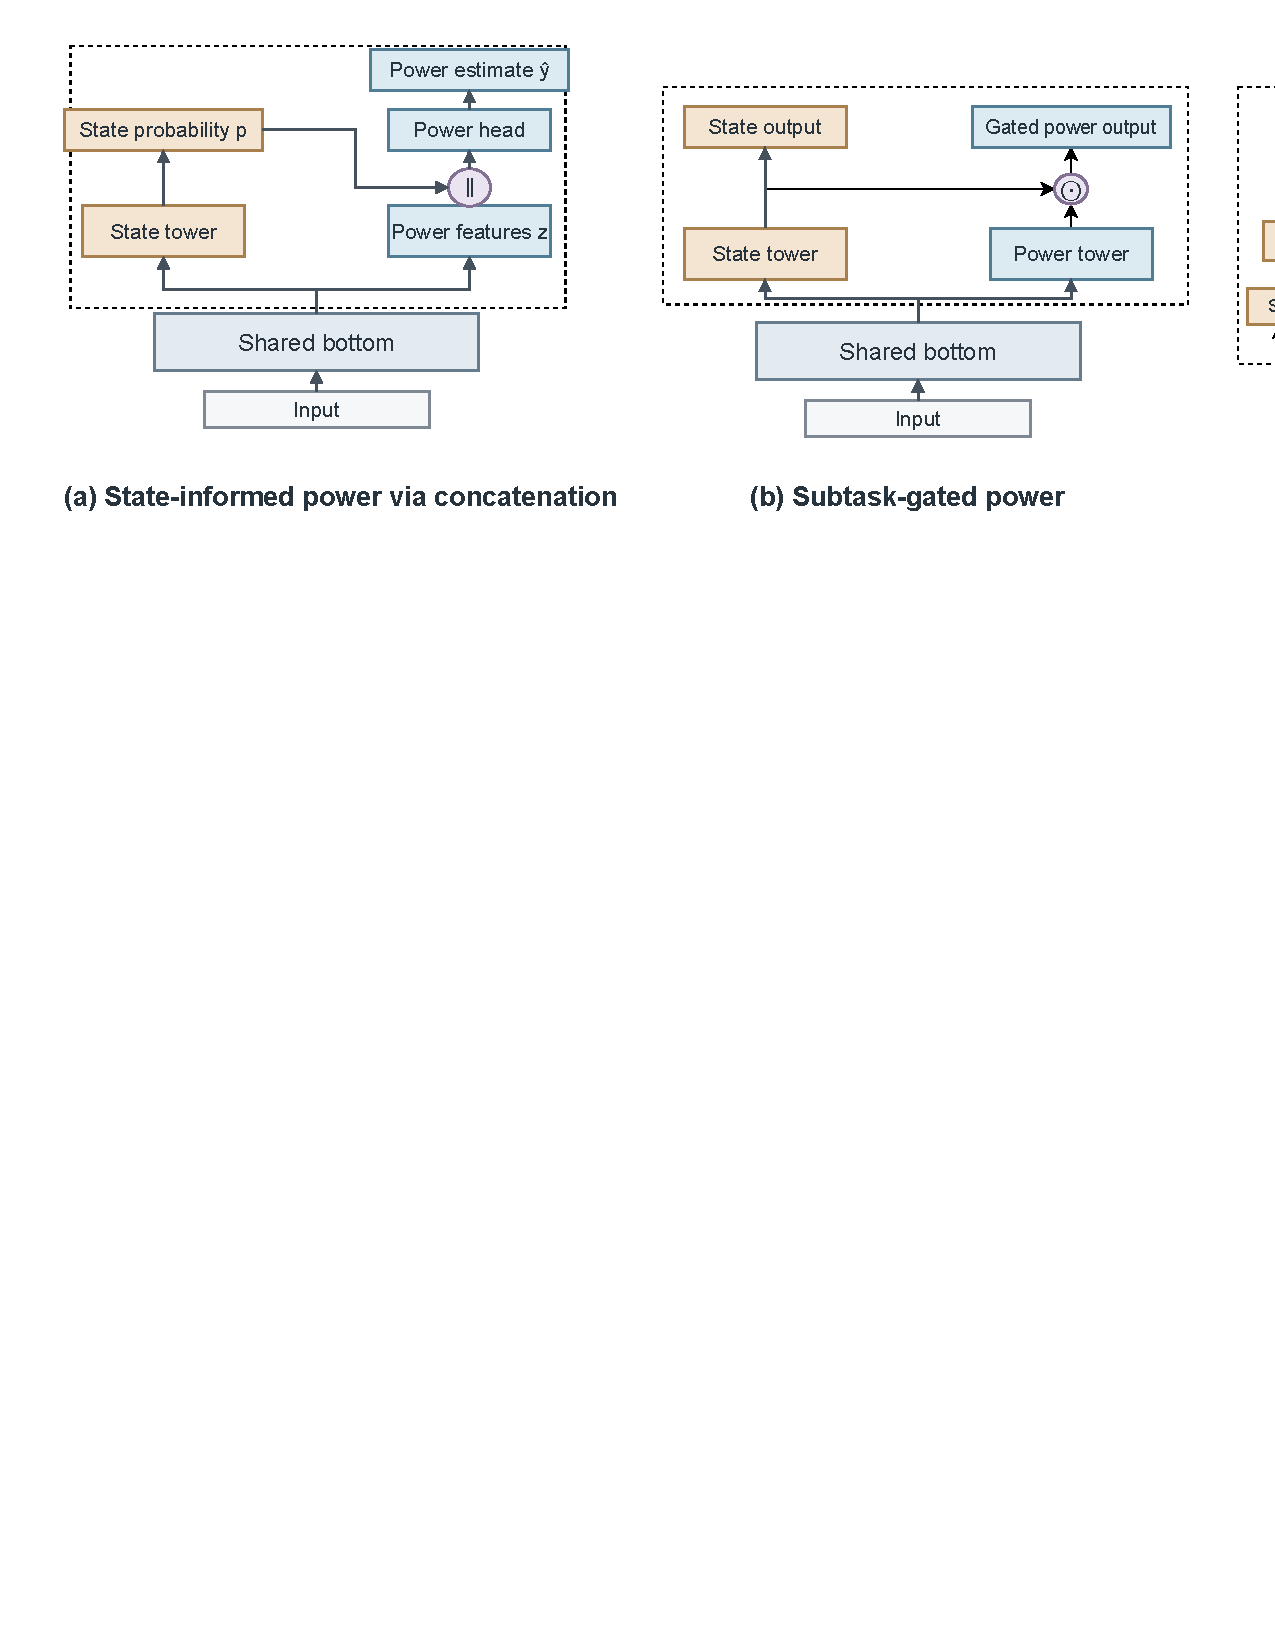
\includegraphics[width=\columnwidth]{figures/appliance_head.pdf}
    \caption{\DIFdelbeginFL \DIFdelFL{Within-appliance power--state }\DIFdelendFL \DIFaddbeginFL \DIFaddFL{Schematic within-appliance power-state }\DIFaddendFL heads: (a) \DIFaddbeginFL \DIFaddFL{state-informed }\DIFaddendFL concatenation \DIFaddbeginFL \DIFaddFL{(Murray \emph{et al.}}\DIFaddendFL ~\cite{murray2019transferability}\DIFdelbeginFL \DIFdelFL{, }\DIFdelendFL \DIFaddbeginFL \DIFaddFL{); }\DIFaddendFL (b) output gating \DIFaddbeginFL \DIFaddFL{(SGN}\DIFaddendFL ~\cite{shin2019sgn}\DIFdelbeginFL \DIFdelFL{, }\DIFdelendFL \DIFaddbeginFL \DIFaddFL{); }\DIFaddendFL and (c) multi-scale fusion \DIFaddbeginFL \DIFaddFL{(SCANet}\DIFaddendFL ~\cite{chen2021sca}\DIFaddbeginFL \DIFaddFL{)}\DIFaddendFL .}
    \label{fig:appliance-head}
\end{figure}

\begin{figure}[!t]
    \centering
    \setlength{\abovecaptionskip}{3pt}
    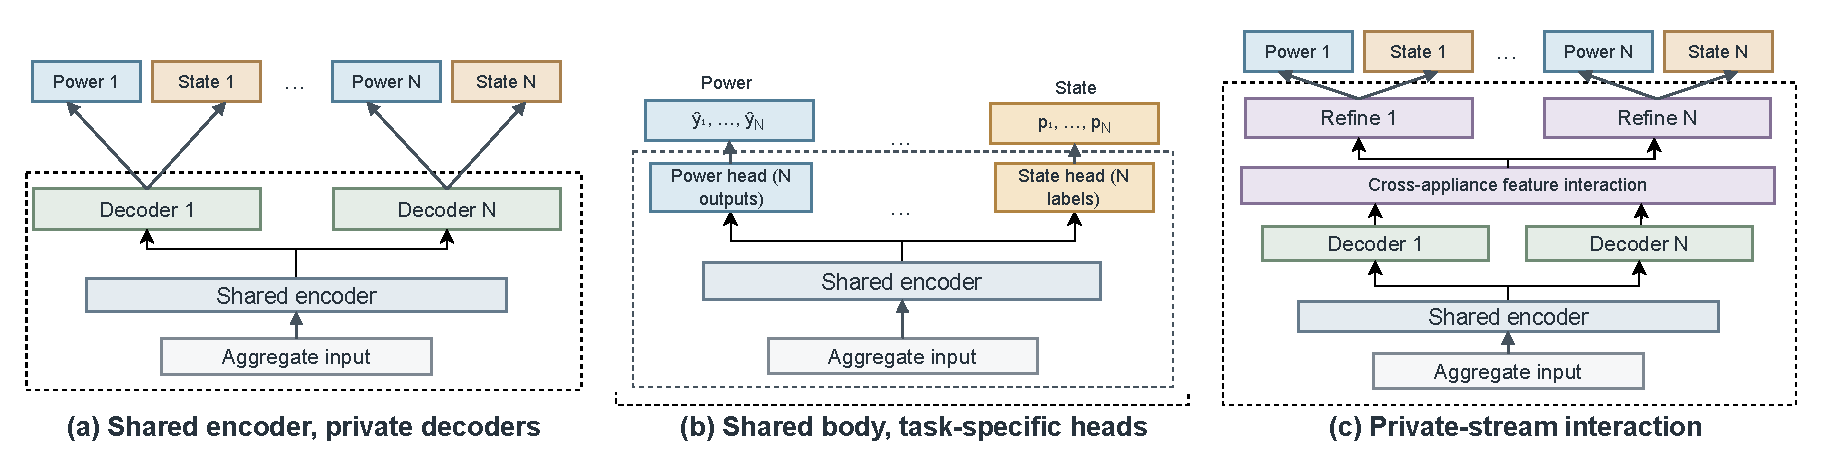
\includegraphics[width=\columnwidth]{figures/model_body_design.pdf}
    \caption{\DIFdelbeginFL \DIFdelFL{Multi-appliance }\DIFdelendFL \DIFaddbeginFL \DIFaddFL{Schematic multi-appliance }\DIFaddendFL body \DIFdelbeginFL \DIFdelFL{designs}\DIFdelendFL \DIFaddbeginFL \DIFaddFL{mechanisms}\DIFaddendFL : (a) shared encoder/private decoders \DIFaddbeginFL \DIFaddFL{(MATNilm}\DIFaddendFL ~\cite{xiong2024matnilm} \DIFdelbeginFL \DIFdelFL{, }\DIFdelendFL \DIFaddbeginFL \DIFaddFL{and Sun \emph{et al.}~\cite{sun2025transfer}); }\DIFaddendFL (b) shared body/task heads \DIFaddbeginFL \DIFaddFL{(UNet-NILM}\DIFaddendFL ~\cite{faustine2020unet}\DIFdelbeginFL \DIFdelFL{, }\DIFdelendFL \DIFaddbeginFL \DIFaddFL{); }\DIFaddendFL and (c) private-stream interaction \DIFaddbeginFL \DIFaddFL{(MATNilm~\cite{xiong2024matnilm} and MART-NILM)}\DIFaddendFL .}
    \label{fig:model-body-design}
\end{figure}

\section{Methodology}
\label{sec:method}

\subsection{Problem Formulation}
\label{sec:problem}

Following \DIFaddbegin \DIFadd{Equation~}\DIFaddend \eqref{eq:aggregate}, \DIFaddbegin \DIFadd{let $\mathbf{x}=(x_1,\ldots,x_T)$ denote an aggregate window of length $T$. The problem is to jointly estimate }\DIFaddend the \DIFdelbegin \DIFdel{model estimates the paired }\DIFdelend power \DIFaddbegin \DIFadd{traces }\DIFaddend and \DIFdelbegin \DIFdel{ON--OFF state outputs }\DIFdelend \DIFaddbegin \DIFadd{ON-state probabilities }\DIFaddend of $N$ target appliances\DIFdelbegin \DIFdel{from an aggregate window $\mathbf{x}$ of length $T$}\DIFdelend :
\DIFdelbegin %DIFDELCMD < \begin{equation}
%DIFDELCMD < f_{\boldsymbol{\theta},t}(\mathbf{x})=
%DIFDELCMD < \underbrace{\bigl(\hat y_{t,1},\hat s_{t,1},\ldots,
%DIFDELCMD < \hat y_{t,N},\hat s_{t,N}\bigr)}_{N\text{ appliance power--state pairs}},
%DIFDELCMD < \quad t=1,\ldots,T.
%DIFDELCMD < \label{eq:paired-outputs}
%DIFDELCMD < \end{equation}%%%
\DIFdelend \DIFaddbegin \begin{equation}
\left(\hat{\mathbf{Y}},\hat{\mathbf{S}}\right)=f_{\boldsymbol{\theta}}(\mathbf{x}),
\qquad
\hat{\mathbf{Y}}\in\mathbb{R}^{T\times N},\quad
\hat{\mathbf{S}}\in[0,1]^{T\times N}
\label{eq:joint-estimation}
\end{equation}\DIFaddend 
Here \DIFdelbegin \DIFdel{$\hat y_{t,i}$ estimates appliance }\DIFdelend \DIFaddbegin \DIFadd{$\boldsymbol{\theta}$ denotes the model parameters, and $\hat{\mathbf{Y}}$ and $\hat{\mathbf{S}}$ collect the estimated }\DIFaddend power \DIFdelbegin \DIFdel{on }\DIFdelend \DIFaddbegin \DIFadd{traces and ON-state probabilities, respectively. To make }\DIFaddend the \DIFdelbegin \DIFdel{standardized scale}\DIFdelend \DIFaddbegin \DIFadd{multi-appliance and multi-label output structure explicit}\DIFaddend , \DIFaddbegin \DIFadd{the time-$t$ output slice of \eqref{eq:joint-estimation} is
}\begin{equation}
f_{\boldsymbol{\theta},t}(\mathbf{x})=
\underbrace{\bigl(\hat y_{t,1},\hat s_{t,1},\ldots,
\hat y_{t,N},\hat s_{t,N}\bigr)}_{N\text{ appliance power-state pairs}},
\quad t=1,\ldots,T.
\label{eq:paired-outputs}
\end{equation}
Power estimation is a regression task, while state detection is formulated as multi-label classification, allowing multiple appliances to be active simultaneously. Binary ON-OFF labels describe appliance activity without distinguishing internal operating modes.

\subsection{Model Architecture}
\label{sec:architecture}

The implementation uses instance-\DIFdelbegin \DIFdel{-}\DIFdelend batch normalization (IBN), batch normalization (BN), the rectified linear unit (ReLU) activation, and fully connected (FC) output layers.

\begin{figure*}[!t]
    \centering
    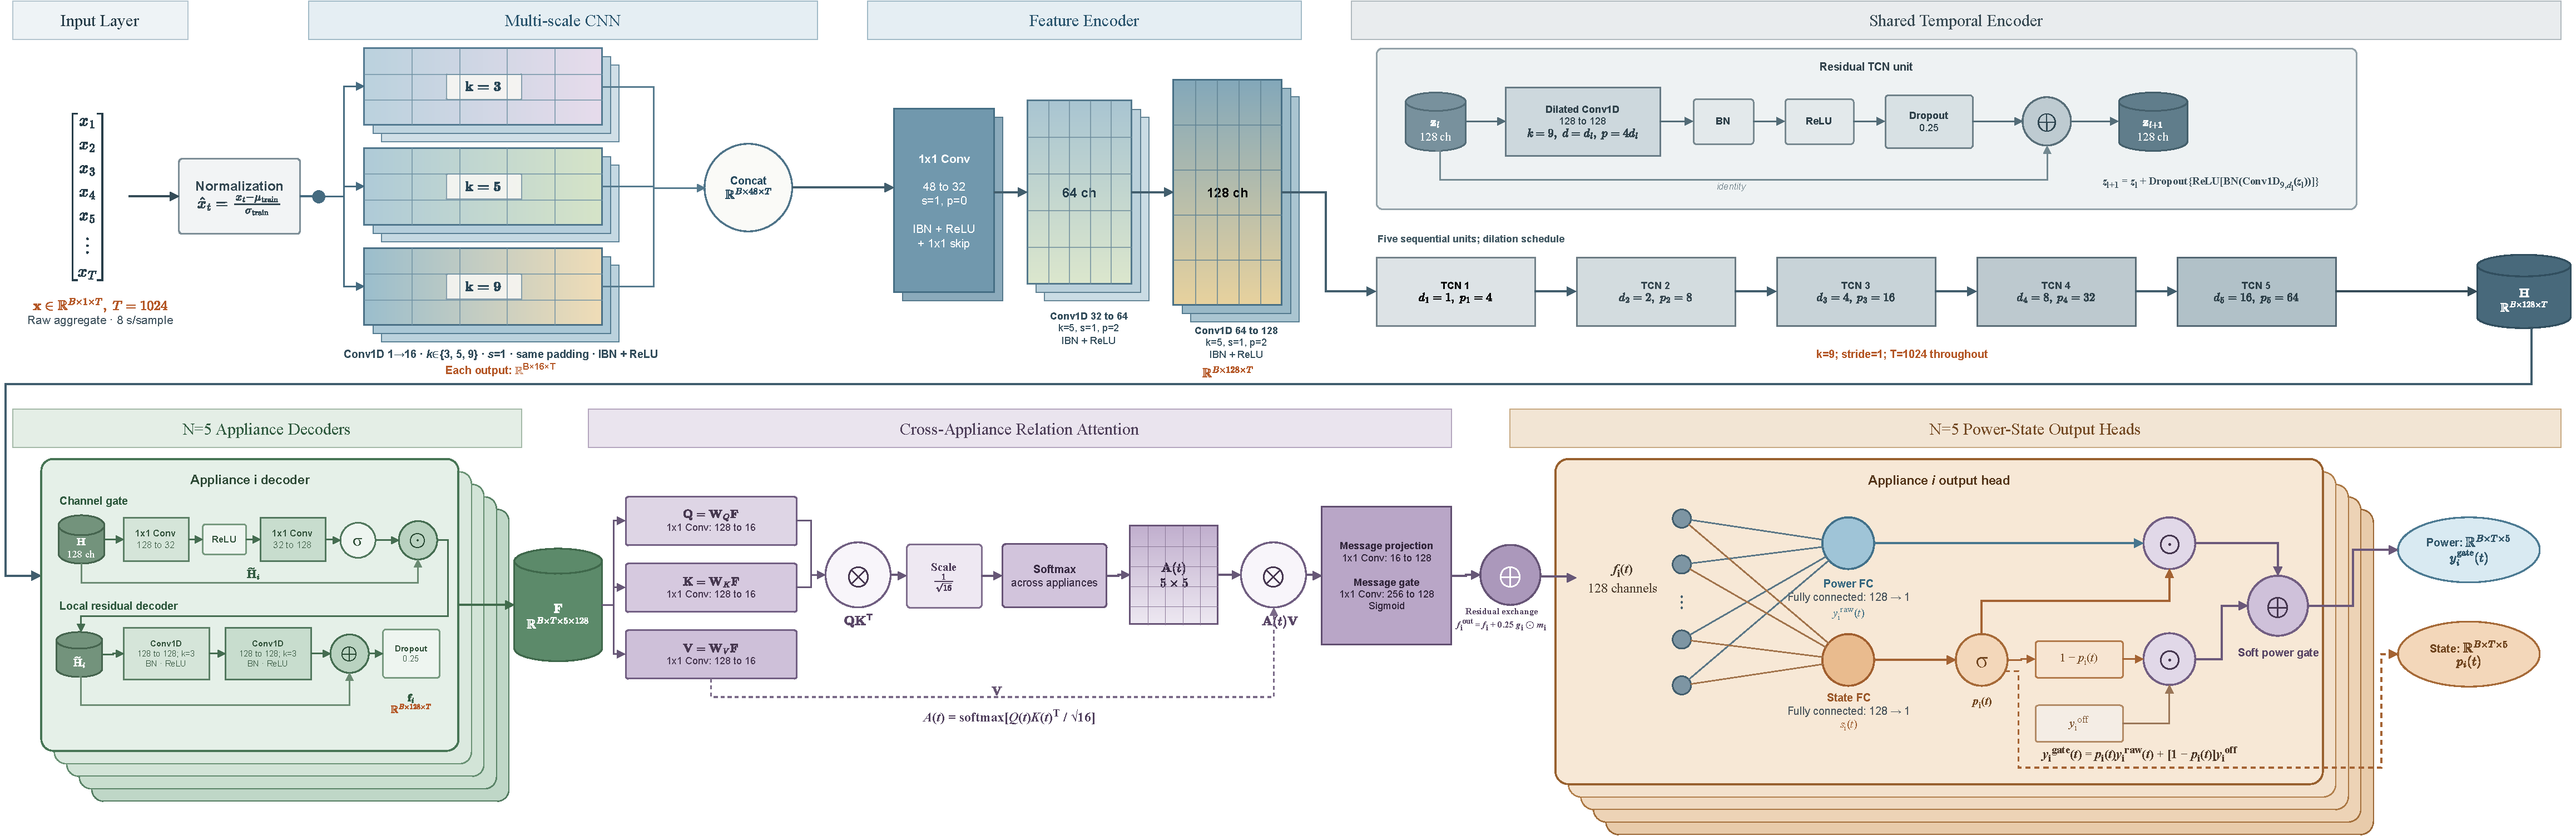
\includegraphics[width=\textwidth]{figures/martnilm_architecture.pdf}
    \caption{Model architecture of MART-NILM.}
    \label{fig:martnilm-architecture}
\end{figure*}

Figure~\ref{fig:martnilm-architecture} presents MART-NILM, combining the private-stream interaction body in Fig.~\ref{fig:model-body-design}(c) with the state-gated heads in Fig.~\ref{fig:appliance-head}(b). The components are described below in processing order, using the same names as the architecture ablations in Table~\ref{tab:architecture-ablation}.

\textit{Multi-scale CNN:}
Parallel convolutional branches~\cite{szegedy2015inception} extract local features at complementary time scales from the standardized aggregate $\bar{\mathbf{x}}$:
\begin{equation}
\mathbf{Z}=\mathcal{F}\!\left(
[\mathcal{B}_{3}(\bar{\mathbf{x}});\mathcal{B}_{5}(\bar{\mathbf{x}});
\mathcal{B}_{9}(\bar{\mathbf{x}})]\right)+\mathcal{S}(\bar{\mathbf{x}}).
\label{eq:multiscale-fusion}
\end{equation}
Here $\mathcal{B}_{k}$ is a kernel-$k$ convolution followed by IBN~\cite{pan2018ibn} and ReLU; $[\cdot;\cdot]$ denotes channel concatenation. The $1\times1$ fusion $\mathcal{F}$ combines the branches, while the projected shortcut $\mathcal{S}$ retains a direct input path. IBN applies instance normalization (IN) and BN to separate channel halves.

\textit{Feature encoder:}
Two \DIFdelbegin \DIFdel{convolution--IBN--ReLU }\DIFdelend \DIFaddbegin \DIFadd{convolution-IBN-ReLU }\DIFaddend stages combine the local features into a shared representation $\mathbf{H}^{(0)}\in\mathbb{R}^{128\times T}$. Feature extraction is performed once for all appliances.

\textit{Temporal encoder:}
Residual dilated TCN blocks~\cite{lea2017tcn} extend temporal context:
\begin{equation}
\mathbf{H}^{(\ell+1)}=\mathbf{H}^{(\ell)}+
\mathcal{T}_{2^{\ell}}(\mathbf{H}^{(\ell)}),
\qquad \ell\in\{0,1,2,3,4\}.
\label{eq:temporal-block}
\end{equation}
Here $\mathcal{T}_{d}$ comprises a dilation-$d$ convolution, BN, ReLU, and dropout. Increasing dilation expands context, while residual connections and symmetric padding retain the incoming features and temporal alignment. The output is $\mathbf{H}=\mathbf{H}^{(5)}$.

\textit{Appliance decoders:}
Each decoder applies a channel gate, inspired by channel recalibration~\cite{hu2018senet}, and a local residual transformation to obtain an appliance-specific representation $\mathbf{F}_i$. These private streams adapt the shared temporal features to individual load characteristics.

\textit{Relation attention:}
The relation module draws on the cross-task information-sharing principle of \DIFaddbegin \DIFadd{the Multi-Tasks Guided Prediction-and-Distillation Network (}\DIFaddend PAD-Net\DIFaddbegin \DIFadd{)}\DIFaddend ~\cite{xu2018padnet} to exchange context among appliance-specific feature streams. Scaled dot-product attention~\cite{vaswani2017attention} is evaluated across appliances at each time $t$:
\begin{equation}
\mathbf{A}_t=\operatorname{softmax}\!\left(
\frac{\mathbf{Q}_t\mathbf{K}_t^{\mathsf T}}{\sqrt{d}}
\right),\qquad
\mathbf{M}_t=\mathbf{A}_t\mathbf{V}_t.
\label{eq:relation-attention}
\end{equation}
Here $\mathbf{Q}_t$, $\mathbf{K}_t$, and $\mathbf{V}_t$ are learned projections of the stacked appliance representations, and $d$ is their projection width. The attended context is projected back to the feature dimension and added to each private stream through a gated residual connection.

\textit{Joint power and state prediction:}
For each appliance, two time-shared FC heads predict raw standardized power $\hat y_i^{\mathrm{raw}}(t)$ and a state logit $a_i(t)$. Following the state-gating principle of SGN~\cite{shin2019sgn}, the \DIFdelbegin \DIFdel{on-state }\DIFdelend \DIFaddbegin \DIFadd{ON-state }\DIFaddend probability $\hat s_i(t)=\operatorname{sigmoid}(a_i(t))$ softly gates the power prediction:
\begin{equation}
\hat y_i(t)=\hat s_i(t)\hat y_i^{\mathrm{raw}}(t)
+[1-\hat s_i(t)]y_i^{(0)},
\label{eq:soft-power-gate}
\end{equation}
where $y_i^{(0)}=-\mu_i/\sigma_i$ is the standardized zero-power anchor. Hence, a low \DIFdelbegin \DIFdel{on-state }\DIFdelend \DIFaddbegin \DIFadd{ON-state }\DIFaddend probability smoothly moves the estimate towards zero power. Predictions are converted back to watts using the appliance training mean $\mu_i$ and standard deviation $\sigma_i$, and negative values are clipped to zero. The gate couples the state and power predictions while retaining a separate waveform regressor.

\subsection{Loss Function}
\label{sec:loss}

The model is trained jointly over all appliances, as in multi-task NILM~\cite{faustine2020unet,xiong2024matnilm,sun2025transfer}. Let $\mathcal{L}_{\mathrm{power},i}$ and $\mathcal{L}_{\mathrm{state},i}$ denote the power and state losses for appliance $i$, respectively. The joint objective is
\begin{equation}
\mathcal{L}=\sum_{i=1}^{N}\left(
\mathcal{L}_{\mathrm{power},i}
+\lambda r_i\mathcal{L}_{\mathrm{state},i}
\right),
\qquad \lambda=0.8.
\label{eq:loss}
\end{equation}
Here $r_i$ is an appliance-wise balancing factor defined below.

\textit{Power loss:}
The power objective combines waveform fidelity \DIFdelbegin \DIFdel{, }\DIFdelend \DIFaddbegin \DIFadd{and }\DIFaddend switching fidelity\DIFdelbegin \DIFdel{, and window-energy consistency}\DIFdelend :
\DIFdelbegin %DIFDELCMD < \begin{equation}
%DIFDELCMD < \mathcal{L}_{\mathrm{power},i}=
%DIFDELCMD < \underbrace{\mathcal{L}_{\mathrm{wave},i}}_{\text{power-level fidelity}}
%DIFDELCMD < +\underbrace{0.15\,\mathcal{L}_{\mathrm{trans},i}}_{\text{transition fidelity}}
%DIFDELCMD < +\underbrace{0.25\,\mathcal{L}_{\mathrm{RE},i}}_{\text{energy consistency}}.
%DIFDELCMD < \label{eq:power-loss}
%DIFDELCMD < \end{equation}%%%
\DIFdelend \DIFaddbegin \begin{equation}
\mathcal{L}_{\mathrm{power},i}=
\underbrace{\mathcal{L}_{\mathrm{wave},i}}_{\text{power-level fidelity}}
+\underbrace{0.15\,\mathcal{L}_{\mathrm{trans},i}}_{\text{transition fidelity}}.
\label{eq:power-loss}
\end{equation}\DIFaddend 
The waveform and transition terms both use mean squared error (MSE), applied to power values and temporal differences, respectively. The expressions below are written for one window; in implementation, \DIFdelbegin \DIFdel{the waveform and transition }\DIFdelend \DIFaddbegin \DIFadd{both }\DIFaddend terms are averaged over the batch and time dimensions\DIFdelbegin \DIFdel{, while the energy term is averaged over windows}\DIFdelend . Let $y_i(t)$ and $\hat y_i(t)$ denote standardized target and predicted power, and let $z_i(t)\in\{0,1\}$ denote the \DIFdelbegin \DIFdel{on--off }\DIFdelend \DIFaddbegin \DIFadd{ON-OFF }\DIFaddend label. For a temporal index set $\mathcal{S}$, define
\begin{equation}
\operatorname{MSE}_{\mathcal{S}}(u,v)=
\frac{1}{\max(|\mathcal{S}|,1)}
\sum_{t\in\mathcal{S}}\bigl(u(t)-v(t)\bigr)^2.
\label{eq:temporal-mse}
\end{equation}
The waveform term evaluates power errors over all samples $\mathcal{T}_0=\{1,\ldots,T\}$, \DIFdelbegin \DIFdel{on-state }\DIFdelend \DIFaddbegin \DIFadd{ON-state }\DIFaddend samples $\mathcal{T}^{\mathrm{on}}_i=\{t\in\mathcal{T}_0:z_i(t)=1\}$, and \DIFdelbegin \DIFdel{off-state }\DIFdelend \DIFaddbegin \DIFadd{OFF-state }\DIFaddend samples $\mathcal{T}^{\mathrm{off}}_i=\{t\in\mathcal{T}_0:z_i(t)=0\}$:
\begin{equation}
\begin{aligned}
\mathcal{L}_{\mathrm{wave},i}={}&
\operatorname{MSE}_{\mathcal{T}_0}(y_i,\hat y_i)
+\operatorname{MSE}_{\mathcal{T}^{\mathrm{on}}_i}(y_i,\hat y_i)\\
&+0.5\,\operatorname{MSE}_{\mathcal{T}^{\mathrm{off}}_i}(y_i,\hat y_i).
\end{aligned}
\label{eq:waveform-loss}
\end{equation}
The first term measures global waveform fidelity; the \DIFdelbegin \DIFdel{on-state }\DIFdelend \DIFaddbegin \DIFadd{ON-state }\DIFaddend term prevents sparse activations from being dominated by \DIFdelbegin \DIFdel{off }\DIFdelend \DIFaddbegin \DIFadd{OFF }\DIFaddend samples, and the lower-weight \DIFdelbegin \DIFdel{off-state }\DIFdelend \DIFaddbegin \DIFadd{OFF-state }\DIFaddend term constrains inactive predictions.

To additionally constrain changes in power, let $\Delta y_i(t)=y_i(t)-y_i(t-1)$ and define $\Delta\hat y_i(t)$ analogously. The transition term compares these differences whenever the appliance is \DIFdelbegin \DIFdel{on }\DIFdelend \DIFaddbegin \DIFadd{ON }\DIFaddend at either adjacent sample, over $\mathcal{T}^{\Delta}_i=\{t\in\{2,\ldots,T\}:z_i(t)=1\ \text{or}\ z_i(t-1)=1\}$:
\begin{equation}
\mathcal{L}_{\mathrm{trans},i}=
\operatorname{MSE}_{\mathcal{T}^{\Delta}_i}(\Delta y_i,\Delta\hat y_i).
\label{eq:transition-loss}
\end{equation}

\DIFdelbegin \DIFdel{Finally, a stabilized relative energy term constrains the window total. With physical-unit powers $P_i(t)=[\sigma_i y_i(t)+\mu_i]_+$ and $\hat P_i(t)=[\sigma_i\hat y_i(t)+\mu_i]_+$, it is
}%DIFDELCMD < \begin{equation}
%DIFDELCMD < \mathcal{L}_{\mathrm{RE},i}=
%DIFDELCMD < \frac{\bigl|\sum_{t=1}^{T}(\hat{P}_i(t)-P_i(t))\bigr|}{\sum_{t=1}^{T}P_i(t)+TP_0},
%DIFDELCMD < \quad P_0=10~\mathrm{W}.
%DIFDELCMD < \label{eq:energy-loss}
%DIFDELCMD < \end{equation}
%DIFDELCMD < %%%
\DIFdel{Here $P_0$ is a stabilizing power scale that limits the weight of near-zero-energy windows while retaining a penalty for false power in all-off windows. The constant sampling interval cancels in the ratio.
}%DIFDELCMD < 

%DIFDELCMD < %%%
\DIFdelend \textit{State loss:}
The state objective combines weighted binary cross-entropy (BCE) with explicit false-positive control:
\begin{equation}
\mathcal{L}_{\mathrm{state},i}=
\underbrace{\mathcal{L}_{\mathrm{BCE},i}}_{\text{class-balanced state detection}}
+\underbrace{\mathcal{L}_{\mathrm{fp},i}}_{\text{false-positive control}}.
\label{eq:state-loss}
\end{equation}
For a mini-batch of $B$ windows, let $\hat s_{b,t,i}\in(0,1)$ be the predicted \DIFdelbegin \DIFdel{on-state }\DIFdelend \DIFaddbegin \DIFadd{ON-state }\DIFaddend probability and $z_{b,t,i}\in\{0,1\}$ the target label. The class-balanced BCE term uses $w_i=\min\{(1-\pi_i)/\pi_i,12\}$, determined by the training \DIFdelbegin \DIFdel{on-state }\DIFdelend \DIFaddbegin \DIFadd{ON-state }\DIFaddend proportion $\pi_i$:
\begin{equation}
\begin{aligned}
\mathcal{L}_{\mathrm{BCE},i}=-\frac{1}{BT}\sum_{b,t}\bigl[&
w_i z_{b,t,i}\log\hat s_{b,t,i}\\
&+(1-z_{b,t,i})\log(1-\hat s_{b,t,i})\bigr].
\end{aligned}
\label{eq:weighted-bce}
\end{equation}
The false-positive term penalizes confident \DIFdelbegin \DIFdel{on-state }\DIFdelend \DIFaddbegin \DIFadd{ON-state }\DIFaddend predictions on \DIFdelbegin \DIFdel{off }\DIFdelend \DIFaddbegin \DIFadd{OFF }\DIFaddend samples:
\begin{equation}
\mathcal{L}_{\mathrm{fp},i}=
\frac{\sum_{b,t}(1-z_{b,t,i})\hat s_{b,t,i}^{2}}{\max\left(\sum_{b,t}(1-z_{b,t,i}),1\right)}.
\label{eq:false-positive-loss}
\end{equation}

\textit{\DIFdelbegin \DIFdel{Appliance-wise task balance}\DIFdelend \DIFaddbegin \DIFadd{Bounded appliance-wise balancing}\DIFaddend :}
To account for the different numerical scales of regression and classification losses, a bounded loss-ratio weighting is used. It is motivated by loss-ratio balancing in SAMNet~\cite{liu2022samnet} and differs from gradient-norm balancing in GradNorm~\cite{chen2018gradnorm}. The global reference ratio $g$ bounds the appliance-specific ratio $r_i$:
\begin{equation}
\begin{aligned}
g&=
\frac{\sum_j\mathcal{L}_{\mathrm{power},j}}{\sum_j\mathcal{L}_{\mathrm{state},j}},\\[-1pt]
r_i&=\min\!\left\{3g,\max\!\left\{
\frac{g}{3},
\frac{\mathcal{L}_{\mathrm{power},i}}{\mathcal{L}_{\mathrm{state},i}}
\right\}\right\}.
\end{aligned}
\label{eq:balanced-ratio}
\end{equation}
At each mini-batch update, $g$ and $r_i$ are evaluated from the current losses and held fixed during back-propagation. The three-fold bounds limit each local ratio to $[g/3,3g]$, preventing extreme weights from dominating optimization.

\subsection{Focal-Event Background-Stratified Mixing}
\label{sec:training-strategy}

Training uses recorded and recomposed aggregate windows with equal probability. Recorded windows preserve the observed joint demand. Recomposed windows extend synthetic aggregate construction in Neural NILM~\cite{kelly2015neural} by pairing appliance events with recorded \DIFdelbegin \DIFdel{residual backgrounds }\DIFdelend \DIFaddbegin \DIFadd{background demand }\DIFaddend from other training windows~\cite{liu2026recomposition}, reducing reliance on house-specific event-\DIFdelbegin \DIFdel{-}\DIFdelend background correlations. For a recorded sequence, the \DIFdelbegin \DIFdel{non-target residual }\DIFdelend \DIFaddbegin \DIFadd{background demand }\DIFaddend is \DIFaddbegin \DIFadd{estimated by the nonnegative residual
}\DIFaddend \begin{equation}
R_t=\left[x_t-\sum_{i=1}^{N}P_{t,i}\right]_+.
\label{eq:training-residual}
\end{equation}
\DIFaddbegin \DIFadd{Here $[u]_+=\max(u,0)$. Unlike $b_t$ in Equation~\eqref{eq:aggregate}, $R_t$ can also include measurement and timing discrepancies. }\DIFaddend For each recomposed window, the residual and appliance traces are drawn from independently selected training windows:
\begin{equation}
\tilde{x}_t=R_t^{(k_0)}+\sum_{i=1}^{N}P_{t,i}^{(k_i)},
\qquad
\tilde{P}_{t,i}=P_{t,i}^{(k_i)},\quad
\tilde{z}_{t,i}=z_{t,i}^{(k_i)},
\label{eq:training-recomposition}
\end{equation}
where $k_0,k_1,\ldots,k_N$ denote independent window indices. One focal appliance $i^\star$ \DIFaddbegin \DIFadd{(the appliance whose sampled window must contain an activation) }\DIFaddend is selected uniformly, and its trace is drawn from a window containing at least one \DIFdelbegin \DIFdel{on }\DIFdelend \DIFaddbegin \DIFadd{ON }\DIFaddend sample. The residual is sampled from a uniformly selected non-empty bin of median residual power, using $[0,100)$, $[100,200)$, $[200,400)$, $[400,800)$, and $[800,\infty)$~W; all remaining appliance traces are sampled independently. Thus, rare events occur against varied recorded backgrounds while their selected power and state labels are retained. Recomposition is used only during training; validation and test use recorded aggregates and aligned labels.

\begin{figure}[!t]
\centering
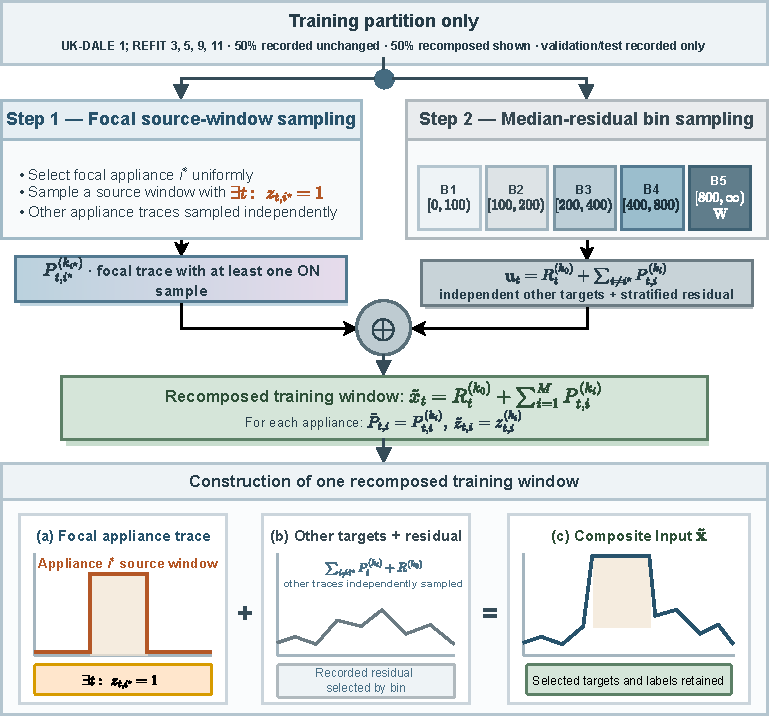
\includegraphics[width=\columnwidth]{figures/focal_event_stratified_mix_crop.pdf}
\caption{Focal-event \DIFdelbeginFL \DIFdelFL{stratified }\DIFdelendFL \DIFaddbeginFL \DIFaddFL{background-stratified }\DIFaddendFL mixing recomposes $\tilde{x}_t$ from an on-event focal trace, a power-stratified residual background, and independently sampled remaining appliance traces.}
\label{fig:focal-mix}
\end{figure}


\section{Experimental Evaluation}
\label{sec:setup}

\subsection{Dataset}
Two public residential datasets are used: the UK Domestic Appliance-Level Electricity (UK-DALE) dataset~\cite{kelly2015ukdale} and the REFIT electrical-load dataset~\cite{murray2017refit}. The target appliances are the kettle, fridge, dishwasher, washer, and microwave, and all signals are resampled at 8~s.

The experiment uses a whole-house split: UK-DALE house 1 and REFIT houses 3, 5, 9, and 11 for training; UK-DALE house 5 and REFIT house 2 for validation; and UK-DALE house 2 and REFIT house 20 for testing. Each house contributes one continuous 5-week block. The held-out blocks are centred within the previously established eight-week recording intervals and are selected without reference to appliance events or model performance. Normalization statistics are estimated from the training houses only.

\subsection{Data Preprocessing}
\label{sec:preprocess}

After 8~s resampling, no additional temporal alignment is applied; residual timing discrepancies remain a measurement limitation. Rows missing any required aggregate, appliance-power, or state-label value are excluded, and windows do not cross timestamp discontinuities.

Let $n$ index windows and $t$ index samples within a window. The aggregate mean and standard deviation, $\mu_x$ and $\sigma_x$, and the corresponding appliance-$i$ statistics, $\mu_i$ and $\sigma_i$, are estimated from the training houses. The input and target powers are standardized as
\begin{equation}
\bar x_{n,t}=\frac{x_{n,t}-\mu_x}{\sigma_x},
\qquad
y_{n,t,i}=\frac{P_{n,t,i}-\mu_i}{\sigma_i}.
\label{eq:power-normalization}
\end{equation}

State labels are precomputed before windowing. For appliances marked in Table~\ref{tab:label}, isolated spikes are first removed on a label-only copy of the resampled power trace. Each sample is then labeled \DIFdelbegin \DIFdel{on }\DIFdelend \DIFaddbegin \DIFadd{ON }\DIFaddend when this trace reaches its appliance-specific threshold $\tau_i^{P}$. OFF gaps of at most $G_i$ are merged; subsequently, complete ON runs shorter than $D_i$ are removed. Runs touching a sequence boundary are retained because their full duration is unobserved. Thus, $\tau_i^{P}$, $G_i$, and $D_i$ denote the ON-power threshold, maximum OFF-gap duration, and minimum ON duration for appliance $i$, respectively. Table~\ref{tab:label} specifies their physical-time values, which are converted to 8~s samples by half-up rounding before labeling. UK-DALE house~5 uses a 30~s fridge gap.

\begin{table}[!t]
\caption{\DIFdelbeginFL \DIFdelFL{ON--OFF }\DIFdelendFL \DIFaddbeginFL \DIFaddFL{ON-OFF }\DIFaddendFL label parameters. The final column lists UK-DALE / REFIT values.}
\label{tab:label}
\centering
\renewcommand{\arraystretch}{1.15}
\footnotesize
\setlength{\tabcolsep}{3pt}
\begin{tabularx}{\linewidth}{@{}l*{3}{>{\centering\arraybackslash}X}@{}}
\hline
Appliance & $\tau^{P}$ (W) & $G$ (s) & $D$ (s) \\
\hline
Kettle & 200 & 0 & 12 / 12 \\
Fridge$^{\dagger}$ & 50 & 12 & 60 / 60 \\
Dishwasher$^{\dagger}$ & 50 & 1800 & 960 / 960 \\
Washer$^{\dagger}$ & 20 & 960 & 960 / 960 \\
Microwave & 200 & 30 & 12 / 6 \\
\hline
\end{tabularx}
\vspace{1pt}
\raggedright\footnotesize $^{\dagger}$ For each sample, a five-sample local-median filter sets its label-generation power to zero when at least 60\% of its four surrounding values are below 50~W and the sample exceeds both three times their median and 100~W. Endpoint windows use edge replication.
\end{table}
\subsection{Experimental Setup}
\label{sec:design}

All experiments were conducted on a single NVIDIA GeForce RTX 4090 graphics processing unit (GPU; 24~GB) using PyTorch~2.6.0 with Compute Unified Device Architecture (CUDA)~12.4. MART-NILM is compared with UNet-NILM~\cite{faustine2020unet}, the convolutional MATNilm variant (MAT-Conv)~\cite{xiong2024matnilm}, and the multi-appliance-task network of Sun \emph{et al.}~\cite{sun2025transfer}. Each baseline retains the architecture, objective, and training hyperparameters of its source paper, while all models use the common \DIFdelbegin \DIFdel{house-held-out }\DIFdelend \DIFaddbegin \DIFadd{cross-house }\DIFaddend data protocol. Table~\ref{tab:cost} lists their settings.

MART-NILM uses weight decay $10^{-4}$ and unit-norm gradient clipping. Its learning rate is reduced by a factor of 0.5 after 12 epochs without validation improvement, to a minimum of $10^{-5}$. Training is limited to 150 epochs; early stopping is disabled before epoch 100 and thereafter uses a patience of 55 epochs. Its 1024-sample input and output windows each cover about 136.5~min.
\begin{table}[!t]
\caption{Training windowing and batch settings. All window lengths and strides are in samples.}
\label{tab:cost}
\centering
\renewcommand{\arraystretch}{1.15}
\footnotesize
\setlength{\tabcolsep}{3pt}
\begin{tabularx}{\linewidth}{@{}l*{6}{>{\centering\arraybackslash}X}@{}}
\hline
Model & Input & Output & Stride & Batch & Optimizer & Epochs \\
\hline
UNet-NILM~\cite{faustine2020unet} & 100 & 1 & 1 & 128 & Adam & 50 \\
MAT-Conv~\cite{xiong2024matnilm} & 864 & 64 & 64 & 64 & Adam & 200 \\
Sun \emph{et al.}~\cite{sun2025transfer} & 480 & 480 & 240 & 32 & Adam & 100 \\
MART-NILM & 1024 & 1024 & 512 & 64 & Adam & 150 \\
\hline
\end{tabularx}
\end{table}

For MART-NILM, checkpoint selection uses only the validation houses. \DIFdelbegin \DIFdel{Normalized mean }\DIFdelend \DIFaddbegin \DIFadd{Mean }\DIFaddend absolute error (MAE) \DIFaddbegin \DIFadd{in standardized power coordinates }\DIFaddend and average precision (AP) are computed from the validation outputs, and the retained checkpoint minimizes
\begin{equation}
S_{\mathrm{val}}=\mathrm{MAE}^{\mathrm{norm}}_{\mathrm{val}}
+1-\mathrm{AP}^{\mathrm{macro}}_{\mathrm{val}},
\label{eq:checkpoint-score}
\end{equation}
where $\mathrm{MAE}^{\mathrm{norm}}_{\mathrm{val}}$ is the macro mean
absolute error over appliances in standardized power coordinates, and the AP
term summarizes the precision-\DIFdelbegin \DIFdel{-}\DIFdelend recall curve without selecting a decision
threshold. For each model and appliance $i$, let
$\hat s_{t,i}\in[0,1]$ denote the predicted ON probability at sample $t$.
After checkpoint selection, an appliance-specific threshold
$\gamma_i\in\{0.05,0.06,\ldots,0.98\}$ is selected on the validation houses to
maximize appliance-level F1 after fixed temporal post-processing is
applied. At test time, the decoded state label is
\begin{equation}
\hat z_{t,i}=\mathbb{I}[\hat s_{t,i}\geq\gamma_i],
\label{eq:state-decoding}
\end{equation}
where $\mathbb{I}[\cdot]$ is the indicator function. For the microwave, fixed
temporal post-processing removes predicted ON runs shorter than 32~s and merges OFF gaps
of at most 24~s. The decoded state is also applied to the power output,
$\hat P^{\mathrm{eval}}_{t,i}=\hat z_{t,i}\hat P_{t,i}$. Thresholds and
temporal rules are frozen before testing and applied unchanged to both test
houses; test labels are not used to select $\gamma_i$.

\subsection{Evaluation Metrics}
\label{sec:metrics}

Each appliance is evaluated on power and on the ON-OFF state. For an evaluated record of length $T_{\mathrm{rec}}$, $P_t$ is the recorded power in watts and $\hat P_t^{\mathrm{eval}}$ is the state-decoded prediction. The label $z_t$ equals 1 when the appliance is recorded ON and 0 when it is OFF. $\hat z_t$ is the predicted label.

Metrics are computed separately for the held-out UK-DALE house~2 and REFIT house~20. Within each test house, the average (Avg.) column is the macro average over the five appliances; architecture-ablation summaries give the two houses equal weight. Performance metrics are reported as mean $\pm$ standard deviation over three random seeds on the fixed cross-house split, so the standard deviation reflects optimization variability. The evaluation considers complementary power-estimation and state-detection metrics.

\subsubsection{Power}
Power error is reported using MAE, ON-state MAE (ON MAE), and blockwise signal aggregate error (SAE). MAE uses every sample; ON MAE is the same quantity evaluated only at samples with $z_t=1$, so that reconstruction quality during appliance operation remains visible:
\begin{equation}
\mathrm{MAE}=\frac{1}{T_{\mathrm{rec}}}\sum_{t=1}^{T_{\mathrm{rec}}}\left|P_t-\hat P_t^{\mathrm{eval}}\right|.
\label{eq:mae}
\end{equation}
Following MATNilm~\cite{xiong2024matnilm}, SAE measures the mean absolute error of average power over $K=\lfloor T_{\mathrm{rec}}/L\rfloor$ non-overlapping 160~min blocks ($L=1200$ samples):
\begin{equation}
\mathrm{SAE}=\frac{1}{K}\sum_{k=1}^{K}\left|\frac{1}{L}\sum_{t=(k-1)L+1}^{kL}\left(P_t-\hat P_t^{\mathrm{eval}}\right)\right|,
\label{eq:sae}
\end{equation}

\subsubsection{On-Off State}
The recorded label $z_t$ follows the rules in Table~\ref{tab:label}, and $\hat{z}_t$ is the predicted binary state. For each appliance, $\mathrm{TP}$ (true positives) counts samples correctly identified as ON ($z_t=1, \hat{z}_t=1$), $\mathrm{FP}$ (false positives) counts inactive samples falsely detected as ON ($z_t=0, \hat{z}_t=1$), and $\mathrm{FN}$ (false negatives) counts active samples missed as OFF ($z_t=1, \hat{z}_t=0$):
\begin{equation}
\mathrm{Precision}=\frac{\mathrm{TP}}{\mathrm{TP}+\mathrm{FP}},\qquad
\mathrm{Recall}=\frac{\mathrm{TP}}{\mathrm{TP}+\mathrm{FN}}.
\label{eq:precision}
\end{equation}
\begin{equation}
\mathrm{F1}=\frac{2\cdot\mathrm{Precision}\cdot\mathrm{Recall}}{\mathrm{Precision}+\mathrm{Recall}}.
\label{eq:f1}
\end{equation}
Precision is the fraction of predicted ON samples that are truly ON, and recall is the fraction of actual ON samples detected. F1 is their harmonic mean; true negatives ($\mathrm{TN}$, $z_t=0, \hat{z}_t=0$) are excluded to prevent long idle background periods from artificially inflating the score.
To evaluate state ranking independently of the calibrated decision threshold, we also report AP from the continuous state probability. Let $\mathcal{P}_n$ and $\mathcal{R}_n$ denote precision and recall after the $n$th distinct probability threshold, with $\mathcal{R}_0=0$. The non-interpolated AP is
\begin{equation}
\mathrm{AP}=\sum_n\left(\mathcal{R}_n-\mathcal{R}_{n-1}\right)\mathcal{P}_n.
\label{eq:average-precision}
\end{equation}
Unlike F1, AP does not use the appliance-specific threshold or the temporal state post-processing fitted on the validation houses.

\section{Results and Discussion}

\subsection{Joint Power and State Estimation}
\label{sec:power-state}

Table~\ref{tab:results} compares joint power-estimation and ON-OFF state-detection performance on the two held-out test houses. A displayed zero standard deviation indicates a value below the shown precision.

\begin{table*}[!t]
\begingroup
\renewcommand{\mstd}[2]{{\fontsize{5.4}{5.9}\selectfont #1$\pm$#2}}
\renewcommand{\bestmstd}[2]{{\fontsize{5.4}{5.9}\selectfont\bfseries #1$\boldsymbol{\pm}$#2}}
\caption{Power and ON-OFF results (mean $\pm$ standard deviation over three seeds; MAE, ON MAE, and SAE are in W). Bold denotes the best displayed mean, including ties.}
\label{tab:results}
\centering
\renewcommand{\arraystretch}{1.08}
\fontsize{6.0}{6.6}\selectfont
\setlength{\tabcolsep}{1.5pt}
\begin{tabularx}{\textwidth}{@{}>{\raggedright\arraybackslash\fontsize{5.0}{5.5}\selectfont}p{0.24in}>{\raggedright\arraybackslash\fontsize{5.0}{5.5}\selectfont}p{0.48in}|*{6}{>{\centering\arraybackslash}X}|*{6}{>{\centering\arraybackslash}X}@{}}
\hline
\multirow{2}{*}{Metric} & \multirow{2}{*}{Method}
 & \multicolumn{6}{c|}{UK-DALE} & \multicolumn{6}{c}{REFIT} \\
\cline{3-14}
 & & Kettle & Fridge & Dishwasher & Washer & Microwave & Avg.
 & Kettle & Fridge & Dishwasher & Washer & Microwave & Avg. \\
\hline
\multirow{4}{*}{MAE}
 & UNet-NILM & \mstd{9.2}{2.1} & \mstd{29.1}{0.9} & \mstd{22.6}{5.1} & \mstd{9.1}{0.1} & \mstd{6.1}{0.3} & \mstd{15.2}{1.1} & \mstd{8.6}{0.9} & \mstd{35.0}{1.7} & \mstd{12.1}{1.1} & \mstd{7.6}{0.1} & \mstd{7.4}{0.3} & \mstd{14.2}{0.3} \\
 & MAT-Conv & \mstd{5.5}{1.6} & \bestmstd{18.4}{0.7} & \mstd{8.9}{2.1} & \mstd{9.6}{1.4} & \mstd{5.3}{0.4} & \mstd{9.5}{1.1} & \bestmstd{5.4}{0.4} & \mstd{40.8}{0.1} & \mstd{5.4}{0.8} & \mstd{6.2}{2.3} & \bestmstd{6.0}{0.7} & \mstd{12.8}{0.6} \\
 & Sun \emph{et al.} & \mstd{8.8}{1.7} & \mstd{34.4}{3.0} & \mstd{14.7}{6.2} & \mstd{15.5}{5.0} & \mstd{6.3}{0.1} & \mstd{15.9}{1.3} & \mstd{10.9}{1.6} & \mstd{35.6}{1.8} & \mstd{9.0}{1.2} & \mstd{18.0}{7.3} & \mstd{6.7}{0.1} & \mstd{16.1}{0.8} \\
 & \textbf{MART-NILM} & \DIFdelbeginFL %DIFDELCMD < \bestmstd{3.8}{0.3} %%%
\DIFdelendFL \DIFaddbeginFL \bestmstd{3.8}{0.2} \DIFaddendFL & \DIFdelbeginFL %DIFDELCMD < \mstd{20.3}{0.4} %%%
\DIFdelendFL \DIFaddbeginFL \mstd{19.8}{0.7} \DIFaddendFL & \DIFdelbeginFL %DIFDELCMD < \bestmstd{4.4}{0.4} %%%
\DIFdelendFL \DIFaddbeginFL \bestmstd{4.2}{0.4} \DIFaddendFL & \bestmstd{5.3}{0.3} & \bestmstd{3.4}{0.1} & \DIFdelbeginFL %DIFDELCMD < \bestmstd{7.5}{0.1} %%%
\DIFdelendFL \DIFaddbeginFL \bestmstd{7.3}{0.2} \DIFaddendFL & \DIFdelbeginFL %DIFDELCMD < \mstd{5.7}{0.1} %%%
\DIFdelendFL \DIFaddbeginFL \mstd{5.9}{0.1} \DIFaddendFL & \DIFdelbeginFL %DIFDELCMD < \bestmstd{32.6}{1.5} %%%
\DIFdelendFL \DIFaddbeginFL \bestmstd{33.0}{1.2} \DIFaddendFL & \DIFdelbeginFL %DIFDELCMD < \bestmstd{4.8}{0.3} %%%
\DIFdelendFL \DIFaddbeginFL \bestmstd{4.9}{0.2} \DIFaddendFL & \DIFdelbeginFL %DIFDELCMD < \bestmstd{3.6}{0.2} %%%
\DIFdelendFL \DIFaddbeginFL \bestmstd{4.1}{0.8} \DIFaddendFL & \DIFdelbeginFL %DIFDELCMD < \mstd{7.3}{0.4} %%%
\DIFdelendFL \DIFaddbeginFL \mstd{6.8}{0.1} \DIFaddendFL & \DIFdelbeginFL %DIFDELCMD < \bestmstd{10.8}{0.4} %%%
\DIFdelendFL \DIFaddbeginFL \bestmstd{10.9}{0.2} \DIFaddendFL \\
\hline
\multirow{4}{*}{SAE}
 & UNet-NILM & \mstd{8.4}{2.6} & \mstd{24.5}{2.5} & \mstd{21.1}{6.5} & \mstd{9.0}{0.1} & \mstd{6.0}{0.4} & \mstd{13.8}{1.3} & \mstd{5.6}{1.1} & \mstd{25.9}{2.6} & \mstd{9.8}{0.3} & \mstd{7.1}{0.3} & \mstd{7.0}{0.2} & \mstd{11.1}{0.7} \\
 & MAT-Conv & \mstd{4.3}{1.2} & \bestmstd{10.0}{1.0} & \mstd{6.7}{1.4} & \mstd{8.8}{1.3} & \mstd{5.0}{0.4} & \mstd{6.9}{0.8} & \mstd{2.9}{0.3} & \mstd{23.7}{0.6} & \mstd{4.5}{1.0} & \mstd{5.0}{1.8} & \bestmstd{5.2}{0.5} & \mstd{8.3}{0.5} \\
 & Sun \emph{et al.} & \mstd{7.3}{1.4} & \mstd{32.1}{3.5} & \mstd{12.0}{5.9} & \mstd{14.5}{4.9} & \mstd{6.2}{0.1} & \mstd{14.4}{1.4} & \mstd{7.1}{1.1} & \mstd{21.7}{4.4} & \mstd{7.9}{1.3} & \mstd{13.0}{5.5} & \mstd{6.6}{0.0} & \mstd{11.3}{0.7} \\
 & \textbf{MART-NILM} & \DIFdelbeginFL %DIFDELCMD < \bestmstd{2.9}{0.2} %%%
\DIFdelendFL \DIFaddbeginFL \bestmstd{2.9}{0.1} \DIFaddendFL & \DIFdelbeginFL %DIFDELCMD < \mstd{13.6}{0.6} %%%
\DIFdelendFL \DIFaddbeginFL \mstd{12.8}{1.5} \DIFaddendFL & \DIFdelbeginFL %DIFDELCMD < \bestmstd{2.8}{0.5} %%%
\DIFdelendFL \DIFaddbeginFL \bestmstd{2.6}{0.7} \DIFaddendFL & \DIFdelbeginFL %DIFDELCMD < \bestmstd{4.1}{0.5} %%%
\DIFdelendFL \DIFaddbeginFL \bestmstd{4.0}{0.4} \DIFaddendFL & \DIFdelbeginFL %DIFDELCMD < \bestmstd{3.0}{0.1} %%%
\DIFdelendFL \DIFaddbeginFL \bestmstd{2.9}{0.1} \DIFaddendFL & \DIFdelbeginFL %DIFDELCMD < \bestmstd{5.3}{0.1} %%%
\DIFdelendFL \DIFaddbeginFL \bestmstd{5.1}{0.4} \DIFaddendFL & \DIFdelbeginFL %DIFDELCMD < \bestmstd{2.3}{0.2} %%%
\DIFdelendFL \DIFaddbeginFL \bestmstd{2.6}{0.1} \DIFaddendFL & \DIFdelbeginFL %DIFDELCMD < \bestmstd{15.0}{1.6} %%%
\DIFdelendFL \DIFaddbeginFL \bestmstd{15.4}{1.6} \DIFaddendFL & \DIFdelbeginFL %DIFDELCMD < \bestmstd{3.6}{0.1} %%%
\DIFdelendFL \DIFaddbeginFL \bestmstd{3.7}{0.2} \DIFaddendFL & \DIFdelbeginFL %DIFDELCMD < \bestmstd{2.9}{0.2} %%%
\DIFdelendFL \DIFaddbeginFL \bestmstd{3.1}{0.9} \DIFaddendFL & \DIFdelbeginFL %DIFDELCMD < \mstd{5.6}{0.3} %%%
\DIFdelendFL \DIFaddbeginFL \mstd{5.2}{0.1} \DIFaddendFL & \DIFdelbeginFL %DIFDELCMD < \bestmstd{5.9}{0.4} %%%
\DIFdelendFL \DIFaddbeginFL \bestmstd{6.0}{0.2} \DIFaddendFL \\
\hline
\multirow{4}{*}{\shortstack{ON\\MAE}}
 & UNet-NILM & \mstd{1296.5}{443.8} & \mstd{48.4}{4.0} & \mstd{747.7}{180.9} & \mstd{462.6}{7.3} & \mstd{1178.8}{93.3} & \mstd{746.8}{110.0} & \mstd{1289.1}{190.7} & \mstd{63.4}{3.4} & \mstd{398.3}{93.1} & \mstd{306.1}{6.7} & \mstd{1196.7}{58.0} & \mstd{650.7}{59.1} \\
 & MAT-Conv & \mstd{547.5}{180.2} & \bestmstd{22.1}{1.6} & \mstd{206.9}{46.2} & \mstd{385.7}{59.1} & \mstd{946.4}{99.8} & \mstd{421.7}{75.2} & \mstd{850.7}{44.4} & \mstd{46.3}{2.5} & \mstd{208.2}{21.0} & \mstd{195.6}{10.1} & \mstd{1062.2}{90.6} & \mstd{472.6}{29.3} \\
 & Sun \emph{et al.} & \mstd{807.3}{69.1} & \mstd{61.0}{7.1} & \mstd{449.8}{212.8} & \mstd{478.2}{28.0} & \mstd{1215.2}{19.2} & \mstd{602.3}{44.3} & \mstd{1012.0}{65.7} & \mstd{59.1}{6.4} & \mstd{437.1}{91.3} & \mstd{306.7}{17.6} & \mstd{1224.2}{5.6} & \mstd{607.8}{16.5} \\
 & \textbf{MART-NILM} & \DIFdelbeginFL %DIFDELCMD < \bestmstd{388.0}{38.1} %%%
\DIFdelendFL \DIFaddbeginFL \bestmstd{383.4}{15.9} \DIFaddendFL & \DIFdelbeginFL %DIFDELCMD < \mstd{26.8}{1.0} %%%
\DIFdelendFL \DIFaddbeginFL \mstd{25.4}{2.1} \DIFaddendFL & \DIFdelbeginFL %DIFDELCMD < \bestmstd{96.0}{9.6} %%%
\DIFdelendFL \DIFaddbeginFL \bestmstd{87.0}{7.4} \DIFaddendFL & \DIFdelbeginFL %DIFDELCMD < \bestmstd{164.0}{19.2} %%%
\DIFdelendFL \DIFaddbeginFL \bestmstd{161.8}{17.0} \DIFaddendFL & \DIFdelbeginFL %DIFDELCMD < \bestmstd{208.5}{21.1} %%%
\DIFdelendFL \DIFaddbeginFL \bestmstd{218.8}{23.9} \DIFaddendFL & \DIFdelbeginFL %DIFDELCMD < \bestmstd{176.7}{7.7} %%%
\DIFdelendFL \DIFaddbeginFL \bestmstd{175.3}{6.9} \DIFaddendFL & \DIFdelbeginFL %DIFDELCMD < \bestmstd{791.8}{22.3} %%%
\DIFdelendFL \DIFaddbeginFL \bestmstd{785.2}{17.4} \DIFaddendFL & \DIFdelbeginFL %DIFDELCMD < \bestmstd{40.7}{1.9} %%%
\DIFdelendFL \DIFaddbeginFL \bestmstd{40.4}{1.5} \DIFaddendFL & \DIFdelbeginFL %DIFDELCMD < \bestmstd{156.9}{17.9} %%%
\DIFdelendFL \DIFaddbeginFL \bestmstd{139.5}{6.0} \DIFaddendFL & \DIFdelbeginFL %DIFDELCMD < \bestmstd{167.7}{2.2} %%%
\DIFdelendFL \DIFaddbeginFL \bestmstd{155.9}{5.3} \DIFaddendFL & \DIFdelbeginFL %DIFDELCMD < \bestmstd{388.9}{22.6} %%%
\DIFdelendFL \DIFaddbeginFL \bestmstd{429.0}{40.8} \DIFaddendFL & \DIFdelbeginFL %DIFDELCMD < \bestmstd{309.2}{4.6} %%%
\DIFdelendFL \DIFaddbeginFL \bestmstd{310.0}{3.5} \DIFaddendFL \\
\hline
\multirow{4}{*}{AP}
 & UNet-NILM & \mstd{0.908}{0.016} & \mstd{0.873}{0.041} & \mstd{0.580}{0.274} & \mstd{0.866}{0.026} & \mstd{0.535}{0.024} & \mstd{0.753}{0.049} & \mstd{0.653}{0.036} & \mstd{0.657}{0.030} & \mstd{0.269}{0.056} & \mstd{0.654}{0.129} & \mstd{0.136}{0.046} & \mstd{0.474}{0.024} \\
 & MAT-Conv & \mstd{0.968}{0.020} & \mstd{0.951}{0.006} & \mstd{0.868}{0.039} & \mstd{0.555}{0.191} & \bestmstd{0.718}{0.063} & \mstd{0.812}{0.051} & \mstd{0.801}{0.018} & \mstd{0.537}{0.005} & \mstd{0.736}{0.040} & \mstd{0.653}{0.066} & \mstd{0.152}{0.046} & \mstd{0.576}{0.024} \\
 & Sun \emph{et al.} & \mstd{0.930}{0.016} & \mstd{0.915}{0.030} & \mstd{0.838}{0.094} & \mstd{0.207}{0.128} & \mstd{0.514}{0.194} & \mstd{0.681}{0.075} & \mstd{0.660}{0.090} & \mstd{0.641}{0.053} & \mstd{0.615}{0.040} & \mstd{0.123}{0.019} & \mstd{0.160}{0.069} & \mstd{0.440}{0.000} \\
 & \textbf{MART-NILM} & \DIFdelbeginFL %DIFDELCMD < \bestmstd{0.997}{0.001} %%%
\DIFdelendFL \DIFaddbeginFL \bestmstd{0.997}{0.000} \DIFaddendFL & \DIFdelbeginFL %DIFDELCMD < \bestmstd{0.969}{0.001} %%%
\DIFdelendFL \DIFaddbeginFL \bestmstd{0.970}{0.001} \DIFaddendFL & \DIFdelbeginFL %DIFDELCMD < \bestmstd{0.963}{0.002} %%%
\DIFdelendFL \DIFaddbeginFL \bestmstd{0.959}{0.002} \DIFaddendFL & \DIFdelbeginFL %DIFDELCMD < \bestmstd{0.985}{0.008} %%%
\DIFdelendFL \DIFaddbeginFL \bestmstd{0.985}{0.007} \DIFaddendFL & \DIFdelbeginFL %DIFDELCMD < \bestmstd{0.718}{0.033} %%%
\DIFdelendFL \DIFaddbeginFL \bestmstd{0.722}{0.046} \DIFaddendFL & \DIFdelbeginFL %DIFDELCMD < \bestmstd{0.926}{0.008} %%%
\DIFdelendFL \DIFaddbeginFL \bestmstd{0.926}{0.010} \DIFaddendFL & \DIFdelbeginFL %DIFDELCMD < \bestmstd{0.848}{0.008} %%%
\DIFdelendFL \DIFaddbeginFL \bestmstd{0.848}{0.007} \DIFaddendFL & \DIFdelbeginFL %DIFDELCMD < \bestmstd{0.737}{0.025} %%%
\DIFdelendFL \DIFaddbeginFL \bestmstd{0.736}{0.030} \DIFaddendFL & \DIFdelbeginFL %DIFDELCMD < \bestmstd{0.766}{0.009} %%%
\DIFdelendFL \DIFaddbeginFL \bestmstd{0.759}{0.014} \DIFaddendFL & \DIFdelbeginFL %DIFDELCMD < \bestmstd{0.904}{0.033} %%%
\DIFdelendFL \DIFaddbeginFL \bestmstd{0.914}{0.010} \DIFaddendFL & \DIFdelbeginFL %DIFDELCMD < \bestmstd{0.557}{0.045} %%%
\DIFdelendFL \DIFaddbeginFL \bestmstd{0.547}{0.056} \DIFaddendFL & \DIFdelbeginFL %DIFDELCMD < \bestmstd{0.762}{0.018} %%%
\DIFdelendFL \DIFaddbeginFL \bestmstd{0.761}{0.016} \DIFaddendFL \\
\hline
\multirow{4}{*}{Precision}
 & UNet-NILM & \mstd{0.80}{0.09} & \mstd{0.74}{0.09} & \mstd{0.55}{0.19} & \mstd{0.84}{0.09} & \mstd{0.57}{0.07} & \mstd{0.70}{0.03} & \mstd{0.63}{0.08} & \mstd{0.60}{0.12} & \mstd{0.26}{0.06} & \bestmstd{0.89}{0.05} & \mstd{0.18}{0.07} & \mstd{0.51}{0.04} \\
 & MAT-Conv & \mstd{0.82}{0.10} & \mstd{0.76}{0.03} & \mstd{0.47}{0.05} & \mstd{0.61}{0.18} & \bestmstd{0.71}{0.09} & \mstd{0.67}{0.08} & \mstd{0.70}{0.10} & \mstd{0.59}{0.00} & \mstd{0.42}{0.06} & \mstd{0.59}{0.07} & \mstd{0.16}{0.03} & \mstd{0.49}{0.04} \\
 & Sun \emph{et al.} & \mstd{0.74}{0.08} & \mstd{0.87}{0.01} & \mstd{0.51}{0.16} & \mstd{0.22}{0.09} & \mstd{0.55}{0.49} & \mstd{0.58}{0.11} & \mstd{0.57}{0.08} & \mstd{0.63}{0.00} & \mstd{0.54}{0.09} & \mstd{0.14}{0.02} & \mstd{0.37}{0.28} & \mstd{0.45}{0.04} \\
 & \textbf{MART-NILM} & \DIFdelbeginFL %DIFDELCMD < \bestmstd{0.94}{0.02} %%%
\DIFdelendFL \DIFaddbeginFL \bestmstd{0.93}{0.01} \DIFaddendFL & \DIFdelbeginFL %DIFDELCMD < \bestmstd{0.88}{0.01} %%%
\DIFdelendFL \DIFaddbeginFL \bestmstd{0.89}{0.02} \DIFaddendFL & \DIFdelbeginFL %DIFDELCMD < \bestmstd{0.63}{0.06} %%%
\DIFdelendFL \DIFaddbeginFL \bestmstd{0.65}{0.03} \DIFaddendFL & \DIFdelbeginFL %DIFDELCMD < \bestmstd{0.92}{0.02} %%%
\DIFdelendFL \DIFaddbeginFL \bestmstd{0.92}{0.01} \DIFaddendFL & \DIFdelbeginFL %DIFDELCMD < \bestmstd{0.71}{0.00} %%%
\DIFdelendFL \DIFaddbeginFL \bestmstd{0.72}{0.00} \DIFaddendFL & \DIFdelbeginFL %DIFDELCMD < \bestmstd{0.82}{0.01} %%%
\DIFdelendFL \DIFaddbeginFL \bestmstd{0.82}{0.00} \DIFaddendFL & \DIFdelbeginFL %DIFDELCMD < \bestmstd{0.76}{0.01} %%%
\DIFdelendFL \DIFaddbeginFL \bestmstd{0.74}{0.01} \DIFaddendFL & \DIFdelbeginFL %DIFDELCMD < \bestmstd{0.64}{0.00} %%%
\DIFdelendFL \DIFaddbeginFL \bestmstd{0.64}{0.01} \DIFaddendFL & \DIFdelbeginFL %DIFDELCMD < \bestmstd{0.62}{0.04} %%%
\DIFdelendFL \DIFaddbeginFL \bestmstd{0.63}{0.02} \DIFaddendFL & \DIFdelbeginFL %DIFDELCMD < \mstd{0.85}{0.07} %%%
\DIFdelendFL \DIFaddbeginFL \mstd{0.83}{0.07} \DIFaddendFL & \DIFdelbeginFL %DIFDELCMD < \bestmstd{0.43}{0.03} %%%
\DIFdelendFL \DIFaddbeginFL \bestmstd{0.46}{0.02} \DIFaddendFL & \bestmstd{0.66}{0.01} \\
\hline
\multirow{4}{*}{Recall}
 & UNet-NILM & \mstd{0.87}{0.08} & \mstd{0.82}{0.14} & \mstd{0.65}{0.21} & \mstd{0.78}{0.04} & \mstd{0.57}{0.07} & \mstd{0.74}{0.05} & \mstd{0.73}{0.03} & \mstd{0.65}{0.18} & \mstd{0.46}{0.07} & \mstd{0.43}{0.13} & \mstd{0.37}{0.04} & \mstd{0.53}{0.07} \\
 & MAT-Conv & \mstd{0.97}{0.01} & \bestmstd{0.98}{0.02} & \mstd{0.98}{0.02} & \mstd{0.49}{0.18} & \mstd{0.67}{0.13} & \mstd{0.82}{0.02} & \mstd{0.78}{0.03} & \bestmstd{0.93}{0.06} & \bestmstd{0.83}{0.02} & \mstd{0.76}{0.21} & \mstd{0.42}{0.25} & \mstd{0.74}{0.11} \\
 & Sun \emph{et al.} & \mstd{0.92}{0.03} & \mstd{0.94}{0.01} & \mstd{0.89}{0.14} & \mstd{0.56}{0.06} & \mstd{0.08}{0.07} & \mstd{0.68}{0.05} & \mstd{0.75}{0.05} & \mstd{0.78}{0.01} & \mstd{0.77}{0.08} & \mstd{0.50}{0.12} & \mstd{0.03}{0.02} & \mstd{0.57}{0.01} \\
 & \textbf{MART-NILM} & \DIFdelbeginFL %DIFDELCMD < \bestmstd{0.99}{0.00} %%%
\DIFdelendFL \DIFaddbeginFL \bestmstd{1.00}{0.00} \DIFaddendFL & \mstd{0.94}{0.01} & \bestmstd{0.99}{0.01} & \DIFdelbeginFL %DIFDELCMD < \bestmstd{0.97}{0.02} %%%
\DIFdelendFL \DIFaddbeginFL \bestmstd{0.97}{0.01} \DIFaddendFL & \DIFdelbeginFL %DIFDELCMD < \bestmstd{0.91}{0.03} %%%
\DIFdelendFL \DIFaddbeginFL \bestmstd{0.90}{0.02} \DIFaddendFL & \bestmstd{0.96}{0.00} & \DIFdelbeginFL %DIFDELCMD < \bestmstd{0.81}{0.01} %%%
\DIFdelendFL \DIFaddbeginFL \bestmstd{0.82}{0.01} \DIFaddendFL & \DIFdelbeginFL %DIFDELCMD < \mstd{0.79}{0.02} %%%
\DIFdelendFL \DIFaddbeginFL \mstd{0.78}{0.04} \DIFaddendFL & \DIFdelbeginFL %DIFDELCMD < \mstd{0.77}{0.04} %%%
\DIFdelendFL \DIFaddbeginFL \mstd{0.75}{0.03} \DIFaddendFL & \DIFdelbeginFL %DIFDELCMD < \bestmstd{0.85}{0.09} %%%
\DIFdelendFL \DIFaddbeginFL \bestmstd{0.88}{0.03} \DIFaddendFL & \DIFdelbeginFL %DIFDELCMD < \bestmstd{0.76}{0.03} %%%
\DIFdelendFL \DIFaddbeginFL \bestmstd{0.72}{0.04} \DIFaddendFL & \DIFdelbeginFL %DIFDELCMD < \bestmstd{0.80}{0.03} %%%
\DIFdelendFL \DIFaddbeginFL \bestmstd{0.79}{0.02} \DIFaddendFL \\
\hline
\multirow{4}{*}{F1}
 & UNet-NILM & \mstd{0.83}{0.03} & \mstd{0.77}{0.07} & \mstd{0.60}{0.20} & \mstd{0.81}{0.03} & \mstd{0.57}{0.04} & \mstd{0.71}{0.03} & \mstd{0.67}{0.03} & \mstd{0.61}{0.08} & \mstd{0.33}{0.07} & \mstd{0.58}{0.12} & \mstd{0.23}{0.05} & \mstd{0.48}{0.04} \\
 & MAT-Conv & \mstd{0.89}{0.06} & \mstd{0.86}{0.01} & \mstd{0.63}{0.04} & \mstd{0.54}{0.17} & \mstd{0.68}{0.06} & \mstd{0.72}{0.05} & \mstd{0.73}{0.05} & \bestmstd{0.72}{0.02} & \mstd{0.55}{0.05} & \mstd{0.65}{0.06} & \mstd{0.23}{0.08} & \mstd{0.58}{0.02} \\
 & Sun \emph{et al.} & \mstd{0.82}{0.04} & \bestmstd{0.91}{0.00} & \mstd{0.64}{0.14} & \mstd{0.30}{0.09} & \mstd{0.15}{0.13} & \mstd{0.56}{0.05} & \mstd{0.64}{0.03} & \mstd{0.70}{0.00} & \mstd{0.63}{0.05} & \mstd{0.21}{0.01} & \mstd{0.06}{0.04} & \mstd{0.45}{0.00} \\
 & \textbf{MART-NILM} & \DIFdelbeginFL %DIFDELCMD < \bestmstd{0.96}{0.01} %%%
\DIFdelendFL \DIFaddbeginFL \bestmstd{0.96}{0.00} \DIFaddendFL & \bestmstd{0.91}{0.00} & \DIFdelbeginFL %DIFDELCMD < \bestmstd{0.77}{0.04} %%%
\DIFdelendFL \DIFaddbeginFL \bestmstd{0.79}{0.02} \DIFaddendFL & \DIFdelbeginFL %DIFDELCMD < \bestmstd{0.94}{0.02} %%%
\DIFdelendFL \DIFaddbeginFL \bestmstd{0.94}{0.01} \DIFaddendFL & \bestmstd{0.80}{0.01} & \DIFdelbeginFL %DIFDELCMD < \bestmstd{0.88}{0.01} %%%
\DIFdelendFL \DIFaddbeginFL \bestmstd{0.88}{0.00} \DIFaddendFL & \DIFdelbeginFL %DIFDELCMD < \bestmstd{0.79}{0.00} %%%
\DIFdelendFL \DIFaddbeginFL \bestmstd{0.78}{0.01} \DIFaddendFL & \mstd{0.71}{0.01} & \DIFdelbeginFL %DIFDELCMD < \bestmstd{0.69}{0.01} %%%
\DIFdelendFL \DIFaddbeginFL \bestmstd{0.69}{0.00} \DIFaddendFL & \DIFdelbeginFL %DIFDELCMD < \bestmstd{0.85}{0.05} %%%
\DIFdelendFL \DIFaddbeginFL \bestmstd{0.85}{0.03} \DIFaddendFL & \DIFdelbeginFL %DIFDELCMD < \bestmstd{0.55}{0.03} %%%
\DIFdelendFL \DIFaddbeginFL \bestmstd{0.56}{0.03} \DIFaddendFL & \DIFdelbeginFL %DIFDELCMD < \bestmstd{0.72}{0.02} %%%
\DIFdelendFL \DIFaddbeginFL \bestmstd{0.72}{0.00} \DIFaddendFL \\
\hline
\end{tabularx}
\endgroup
\end{table*}

MART-NILM achieves the lowest appliance-average MAE and highest macro-F1 on both test houses among the evaluated models, outperforming MAT-Conv, the strongest baseline in overall performance. Relative to MAT-Conv, MART-NILM reduces overall MAE by $23.6\%$ and $14.5\%$ on UK-DALE and REFIT, respectively. More pronounced improvements are observed during appliance operation, with ON MAE decreasing by $58.4\%$ and $34.4\%$, respectively. Blockwise SAE also decreases by $27.0\%$ and $27.8\%$. State-detection performance improves consistently at the macro level: macro-F1 increases from $0.72$ to $0.88$ on UK-DALE and from $0.58$ to $0.72$ on REFIT. Threshold-independent macro-AP also rises from $0.812$ to $0.926$ and from $0.576$ to $0.761$, respectively, indicating improvements in state-probability ranking beyond the selected decision thresholds. MART-NILM also records the highest mean AP across all ten appliance-dataset combinations, although the margins are small for some appliances. Together with the macro-F1 improvements, these results indicate that the state-detection gains extend beyond threshold selection.

The improvements are not uniform across individual appliances. MAT-Conv retains lower MAE for the UK-DALE fridge and REFIT kettle and microwave, while its REFIT fridge F1 is marginally higher. Nevertheless, the REFIT microwave illustrates the importance of joint power-state evaluation: although MART-NILM has a higher overall MAE ($6.8$ versus $6.0$~W), it substantially reduces ON MAE from $1062.2$ to $429.0$~W and improves F1 from $0.23$ to $0.56$. These appliance-level differences show that the complete framework improves the overall balance between power estimation and state detection, rather than uniformly outperforming the baselines on every metric.

Figure~\ref{fig:baseline-waveforms} provides a qualitative view of the same comparison. MART-NILM generally follows activation boundaries and multi-stage plateaus while suppressing inactive-period power, although amplitude and timing errors remain.

\begin{figure*}[!t]
\centering
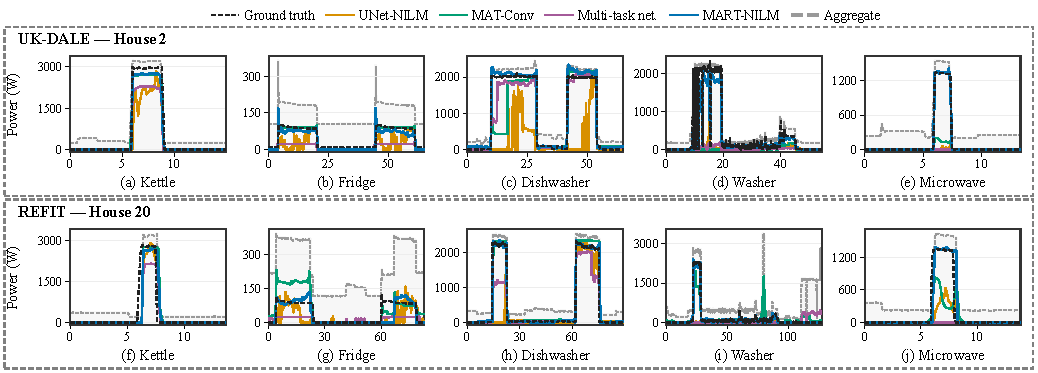
\includegraphics[width=\textwidth]{figures/baseline_waveforms_context.pdf}
\caption{Waveform comparisons on the two test houses.}
\label{fig:baseline-waveforms}
\end{figure*}

\subsection{Performance and Model Efficiency}
\label{sec:cost}

\begin{table}[!t]
\caption{Model size and observed computational cost. M and MB denote millions of parameters and megabytes, respectively.}
\label{tab:time}
\centering
\renewcommand{\arraystretch}{1.15}
\footnotesize
\setlength{\tabcolsep}{2pt}
\begin{tabularx}{\linewidth}{@{}l*{4}{>{\centering\arraybackslash}X}@{}}
\hline
Model & Parameters (M) & Model size (MB) & Training (s) & Inference (s) \\
\hline
UNet-NILM & 5.832 & 22.299 & 17,455.8 & 80.40 \\
MAT-Conv & 3.022 & 11.611 & 10,354.9 & 14.67 \\
Sun \emph{et al.} & 7.829 & 59.793 & 16,493.8 & 23.50 \\
MART-NILM & \textbf{1.373} & \textbf{5.335} & \textbf{485.2} & \textbf{1.14} \\
\hline
\end{tabularx}
\end{table}

Table~\ref{tab:time} shows that MART-NILM uses only $1.373$ million parameters, representing reductions of $54.6\%$, $76.5\%$, and $82.5\%$ relative to MAT-Conv, UNet-NILM, and Sun \emph{et al.}, respectively. Together with the improvements in appliance-average MAE and macro-F1 in Table~\ref{tab:results}, these results demonstrate a favorable accuracy-capacity trade-off: stronger joint prediction performance is achieved with substantially fewer model parameters. MART-NILM also has the smallest checkpoint and the shortest observed training and end-to-end inference times under the evaluated protocols. The complete prediction pipeline processes both test records in $1.14$~s, compared with $14.67$~s for MAT-Conv, $23.50$~s for Sun \emph{et al.}, and $80.40$~s for UNet-NILM. The benchmark includes data transfer and output reconstruction under each model's native windowing protocol, so it measures the complete prediction pipeline rather than isolated forward-pass latency. MART-NILM benefits from producing long output sequences: its 1024-sample windows advance by 512 samples, requiring substantially fewer windows than sequence-to-point inference while preserving dense temporal predictions.

\subsection{Architecture Ablation Study}
\label{sec:ablation}

Each variant in Table~\ref{tab:architecture-ablation} removes or simplifies one top-level component while preserving the joint five-appliance output structure and compatible feature dimensions.

\begin{table}[!t]
\caption{Architecture ablation (three-seed mean $\pm$ standard deviation over the two test houses; MAE, ON MAE, and SAE are in W).}
\label{tab:architecture-ablation}
\centering
\renewcommand{\arraystretch}{1.08}
\fontsize{6.0}{6.8}\selectfont
\setlength{\tabcolsep}{1.2pt}
\begin{tabular*}{\columnwidth}{@{\extracolsep{\fill}}lccccc@{}}
\toprule
Variant & Params (M) & MAE $\downarrow$ & ON MAE $\downarrow$ & SAE $\downarrow$ & Macro-F1 $\uparrow$ \\
\midrule
Single-scale CNN                           & 1.372 & \mstd{9.22}{0.18}  & \mstd{241.75}{8.76}     & \mstd{5.66}{0.17}     & \mstd{0.795}{0.001} \\
Without feature encoder                    & 1.326 & \mstd{9.16}{0.06}  & \mstd{252.01}{2.21}     & \mstd{5.59}{0.07}     & \mstd{0.790}{0.006} \\
Without shared temporal encoder            & 0.634 & \mstd{10.56}{0.33} & \mstd{288.07}{10.25}    & \mstd{6.56}{0.16}     & \mstd{0.710}{0.013} \\
Without appliance decoders                 & 0.836 & \mstd{9.22}{0.66}  & \mstd{265.84}{4.30}     & \mstd{5.63}{0.63}     & \mstd{0.783}{0.015} \\
Without cross-appliance relation attention & 1.332 & \mstd{9.18}{0.09}  & \bestmstd{230.84}{14.69} & \bestmstd{5.55}{0.04} & \mstd{0.790}{0.015} \\
\textbf{MART-NILM}                         & 1.373 & \bestmstd{9.12}{0.14} & \mstd{242.94}{5.35}  & \mstd{5.58}{0.17}     & \bestmstd{0.796}{0.008} \\
\bottomrule
\end{tabular*}
\end{table}

The components make complementary contributions rather than improving every metric uniformly. Temporal modeling has the largest effect: removing it increases MAE by $1.44$~W and lowers macro-F1 from $0.796$ to $0.710$. Removing the appliance-specific decoders increases ON MAE from $242.94$ to $265.84$~W and reduces macro-F1 from $0.796$ to $0.783$. These changes support retaining lightweight appliance-specific refinement alongside the shared temporal encoder. The feature encoder improves all four aggregate measures. Replacing the multi-scale CNN with a single-scale variant slightly worsens MAE, SAE, and macro-F1 while marginally improving ON MAE, indicating a modest rather than uniform contribution.

Cross-appliance relation attention provides a modest improvement in macro-F1 rather than a uniform reduction in power errors. Removing the module lowers macro-F1 from $0.796$ to $0.790$ but slightly improves ON MAE and SAE, indicating a trade-off between state detection and power reconstruction. It also increases the across-seed standard deviation from $5.35$ to $14.69$~W for ON MAE and from $0.008$ to $0.015$ for macro-F1. Thus, cross-appliance exchange does not minimize every power error; it is retained because it improves joint detection and makes the activity-sensitive results more consistent across training runs. The complete model consequently provides the best MAE and macro-F1 rather than the best value for every individual metric.

\subsection{Effects of the Training Strategies}

Table~\ref{tab:training-ablation} evaluates focal-event mixing and appliance-wise balancing independently and jointly with the architecture fixed.

\begin{table}[!t]
\caption{Training-strategy ablation on the validation houses (three-seed mean $\pm$ standard deviation; MAE, ON MAE, and SAE are in W). $\dagger$~denotes a strategy proposed in this work.}
\label{tab:training-ablation}
\centering
\renewcommand{\arraystretch}{1.15}
\footnotesize
\setlength{\tabcolsep}{2pt}
\begin{tabular*}{\columnwidth}{@{\extracolsep{\fill}}lcccc@{}}
\toprule
Training strategy & MAE $\downarrow$ & ON MAE $\downarrow$ & SAE $\downarrow$ & Macro-F1 $\uparrow$ \\
\midrule
\hspace{3pt}Standard joint training       & \mstd{21.164}{0.394} & \mstd{357.808}{19.280} & \mstd{15.938}{0.348} & \mstd{0.605}{0.012} \\
\hspace{3pt}$+$ Focal-event mixing$^\dagger$       & \mstd{21.679}{0.144} & \bestmstd{301.623}{16.196} & \mstd{15.601}{0.365} & \mstd{0.649}{0.016} \\
\hspace{1pt}$+$ Appliance-wise balancing$^\dagger$ & \mstd{20.929}{0.065} & \mstd{334.862}{10.888} & \mstd{15.175}{0.322} & \mstd{0.661}{0.014} \\
\textbf{Complete MART-NILM}$^\dagger$  & \bestmstd{20.791}{0.175} & \mstd{315.408}{10.405} & \bestmstd{15.016}{0.385} & \bestmstd{0.687}{0.003} \\
\bottomrule
\end{tabular*}
\end{table}

Focal-event mixing reduces ON MAE from $357.808$ to $301.623$~W and increases macro-F1 from $0.605$ to $0.649$, while overall MAE rises from $21.164$ to $21.679$~W. This pattern is consistent with the strategy's emphasis on active-appliance exposure rather than uniform improvement across all samples. In contrast, appliance-wise balancing independently improves all four evaluation metrics, reducing MAE from $21.164$ to $20.929$~W while increasing macro-F1 from $0.605$ to $0.661$. Combining both strategies yields the lowest validation MAE ($20.791$~W), lowest SAE ($15.016$~W), and highest macro-F1 ($0.687$). However, focal-event mixing alone retains the lowest ON MAE ($301.623$~W), indicating complementary training effects rather than uniform improvements across all metrics.

\begin{figure*}[!t]
\centering
\begin{minipage}[t]{0.45\textwidth}
\centering
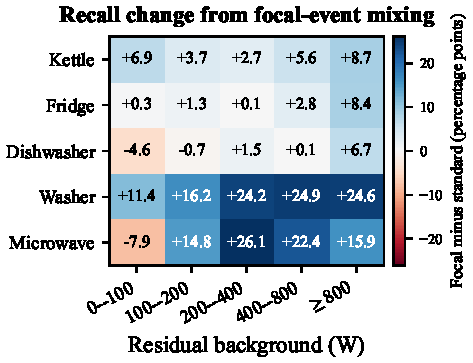
\includegraphics[width=\linewidth]{figures/focal_recall_by_background.pdf}\\[-2pt]
\footnotesize (a)
\end{minipage}\hspace{0.03\textwidth}
\begin{minipage}[t]{0.45\textwidth}
\centering
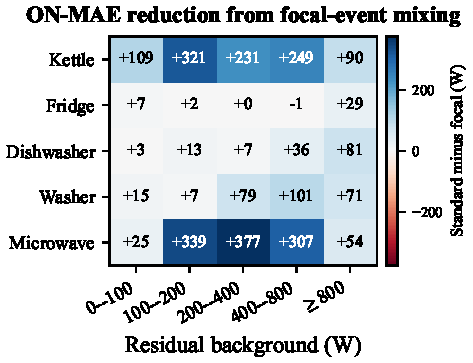
\includegraphics[width=\linewidth]{figures/focal_on_mae_by_background.pdf}\\[-2pt]
\footnotesize (b)
\end{minipage}
\caption{Effect of focal-event mixing across validation background-demand intervals: (a) active-state recall change in percentage points; (b) ON MAE reduction in watts. Positive values indicate improvement.}
\label{fig:focal-background}
\end{figure*}

Figure~\ref{fig:focal-background} examines performance across different residual-background power levels. Focal-event mixing improves kettle and microwave reconstruction in several background strata, while washer recall increases across most evaluated intervals. However, performance deteriorates in some low-background conditions, indicating that the benefits are background-dependent rather than uniform across all operating conditions.

\begin{figure}[!t]
\centering
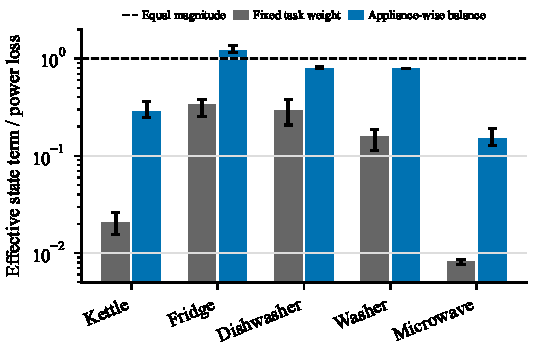
\includegraphics[width=0.90\columnwidth]{figures/appliance_balance_scale.pdf}
\caption{Power-state scale alignment produced by appliance-wise balancing. Bars show the median effective state-term-to-power-loss ratio pooled over epochs 20 onward and three seeds; error bars denote the interquartile range.}
\label{fig:balance-scale}
\end{figure}

\begingroup
\interlinepenalty=10000
Figure~\ref{fig:balance-scale} illustrates the numerical effect of appliance-wise loss balancing. Under fixed weighting, the median state-loss contribution represents only $2.0\%$ and $0.8\%$ of the corresponding power loss for kettle and microwave, respectively. Bounded appliance-wise balancing increases these ratios to $28.5\%$ and $15.1\%$, reducing the numerical disparity between the two objectives. These changes are consistent with the validation improvements in Table~\ref{tab:training-ablation}, although they do not establish equivalent gradient contributions.
\par
\endgroup

\subsection{Limitations and Future Work}

The remaining limitations concern microwave detection and sensitivity to the background-demand level. In the training-strategy ablation, microwave F1 changes from $0.352\pm0.026$ to $0.348\pm0.027$, so no detection gain is claimed. Earlier neural and multi-appliance studies likewise report weaker or highly variable microwave performance~\cite{kelly2015neural,faustine2020unet,xiong2024matnilm}, while SAMNet shows that similar-power background loads can be mistaken for the target appliance~\cite{liu2022samnet}. Short, intermittent, and variable-power activations compound this ambiguity. Focal-event mixing mitigates microwave errors across several background-demand conditions in Fig.~\ref{fig:focal-background} but does not eliminate them. Under high aggregate demand, overlapping non-target activity can obscure appliance transitions even when the target signature is unchanged. Domain variation in NILM should therefore encompass both appliance-signature shifts and changes in household background-demand composition. Future work should model these sources jointly across houses and regions rather than treating appliance waveform variation alone.

\section{Conclusion}

This paper presented MART-NILM, a compact framework for joint multi-appliance power estimation and multi-label ON-OFF state detection from low-frequency aggregate measurements. The architecture combines shared temporal encoding, appliance-specific refinement, and cross-appliance feature exchange, while two training-only strategies address limited event-background coverage and appliance-specific power-state loss imbalance. On the held-out UK-DALE and REFIT test houses, MART-NILM achieves appliance-average MAEs of $7.3$ and $10.9$~W and macro-F1 scores of $0.88$ and $0.72$, respectively. Relative to MAT-Conv, the strongest reproduced baseline in overall performance, ON MAE decreases by $58.4\%$ and $34.4\%$ across the two datasets, while the proposed model uses $54.6\%$ fewer parameters. Architecture ablations highlight the importance of shared temporal modeling and appliance-specific refinement, while training-strategy ablations reveal complementary effects on active-state reconstruction and overall joint prediction. Together, these findings support compact joint power-state estimation as a smart-meter observation layer for residential demand-side monitoring.

\bibliographystyle{IEEEtran}
\bibliography{references/references}

\end{document}
